% Préambule
\documentclass[a4paper, 12pt, twoside]{book}

% Paquets obligatoires
\usepackage{lmodern}
\usepackage[english, french]{babel}
\usepackage[utf8]{inputenc}
\usepackage[T1]{fontenc}
\usepackage[pdfusetitle, pdfsubject={Mémoire TNAH BENIERE 2023}]{hyperref}
    \hypersetup{colorlinks=true, linkcolor=black, urlcolor=blue, citecolor=black}

% Configuration de la mise en page
\usepackage[margin=2.5cm]{geometry}  % Marges du document
\usepackage{parskip}  % Espacement entre les paragraphes
    \parskip=6pt
\usepackage{setspace}  % Mise en forme des paragraphes
    \onehalfspacing
    \setlength\parindent{1cm}

% Configuration de la bibliographie
\usepackage[backend=biber, sorting=nyt, style=enc]{biblatex}
\usepackage[autostyle]{csquotes}
\addbibresource{bibliographie.bib}
\nocite{*}

% Paquets additionnels
\usepackage{xcolor}  % Gestion des couleurs
\usepackage{graphicx}  % Gestion des images
\usepackage{fancyhdr}  % Gestion de l'en-tête et du pied de page
    \pagestyle{headings}
    \pagestyle{fancy}
    \fancyhf{}
    \fancyhead[LE,RO]{\thepage}
    \fancyhead[LO,RE]{\leftmark}
    \setlength{\headheight}{15.5pt}
    \setcounter{secnumdepth}{3}
    \setcounter{tocdepth}{3}
\usepackage{emptypage}  % Gestion des pages vierges
\usepackage{pdfpages}  % Gestion des PDF
\usepackage{shorttoc}  % Gestion du sommaire
\usepackage{array,multirow,makecell}  % Gestion des tableaux
    \setcellgapes{1pt}
    \makegapedcells
    \newcolumntype{R}[1]{>{\raggedleft\arraybackslash }b{#1}}
    \newcolumntype{L}[1]{>{\raggedright\arraybackslash }b{#1}}
    \newcolumntype{C}[1]{>{\centering\arraybackslash }b{#1}}
\usepackage{minted}  % Gestion du code
    \usemintedstyle{perldoc}

% Configuration du point médian
\def\cdt{\kern-0.5pt\ensuremath\cdot\kern-0.5pt}

\author{Sarah Bénière - M2 TNAH}
\title{De l'encodage à la publication : les éditions en ligne de la \textit{European Holocaust Research Infrastructure} et leur chaîne éditoriale}

% Mémoire
\begin{document}
    \begin{titlepage}
		\begin{center}
			
			\bigskip
			
			\begin{large}				
				ÉCOLE NATIONALE DES CHARTES\\
				UNIVERSITÉ PARIS, SCIENCES \& LETTRES
			\end{large}
			\begin{center}\rule{2cm}{0.02cm}\end{center}
			
			\bigskip
			\bigskip
			\bigskip
			
			\begin{Large}
				\textbf{Sarah Bénière}\\
			\end{Large}
			\begin{normalsize} \textit{licenciée ès lettres}\\
				\textit{diplômée de master}
			\end{normalsize}
			
			\bigskip
			\bigskip
			\bigskip
			
			\begin{Huge}
				\textbf{De l'encodage à la publication :}\\
			\end{Huge}
			\bigskip
			\bigskip
			\begin{LARGE}
				\textbf{Les éditions en ligne de la \textit{European Holocaust Research Infrastructure} et leur chaîne éditoriale}\\
			\end{LARGE}
			
			\bigskip
			\bigskip
			\bigskip

            \begin{figure}[h]
                \centering
                
\includegraphics[width=0.5\linewidth]{1-FRONT//images/logo-ehri.jpg}
                \label{fig:logo-ehri}
            \end{figure}
   
			\vfill
			
			\begin{large}
				Mémoire 
				pour le diplôme de master \\
				\og{} Technologies numériques appliquées à l'histoire \fg{} \\
				\bigskip
				2023
			\end{large}
		\end{center}
	\end{titlepage}

    \thispagestyle{empty}
    \cleardoublepage

    \frontmatter
    % Résumé du mémoire
    \chapter{Résumé}
    \medskip
    Le projet EHRI (\textit{European Holocaust Research Infrastructure}) a pour objectif de promouvoir la recherche sur la Shoah, notamment grâce à la publication en ligne de documents d'archives sous la forme d'éditions thématiques. Le présent mémoire rend compte du développement du modèle d'encodage de ces éditions, à partir des collections déjà publiées, et propose un aperçu de leur publication avec l'outil TEI Publisher.

    % Mots-clés
    \bigskip
    \textbf{Mots-clés~:} Édition numérique~; XML-TEI~; ODD~; Modèle d'encodage~; TEI Publisher~; Histoire de la Shoah.

    % Informations bibliographiques
    \bigskip
    \textbf{Informations bibliographiques~:} Sarah Bénière, \textit{De l'encodage à la publication : les éditions en ligne de la European Holocaust Research Infrastructure et leur chaîne éditoriale}, mémoire de master \enquote{Technologies numériques appliquées à l'histoire}, dir. Floriane Chiffoleau et Jean-Damien Généro, École nationale des chartes, 2023.

    \newpage{\pagestyle{empty}\cleardoublepage}

    % Remerciements
    \chapter{Remerciements}
    % Remerciements

Je souhaite remercier toute l'équipe d'ALMAnaCH pour leur accueil, et auprès de qui j'ai beaucoup appris. Je tiens à remercier en particulier Floriane Chiffoleau, ma tutrice, pour son encadrement, ses conseils et son soutien. J'adresse également mes remerciements à mon directeur de mémoire, Jean-Damien Généro, pour son aide précieuse et ses conseils.  

Je remercie chaleureusement mes camarades et amies Jade et Maëva, pour toute leur aide, leur soutien et leur présence au cours de ces deux dernières années. J'adresse également mes remerciements à mon entourage d'Aix-en-Provence, en particulier à Prudence, Aurélia, Manon et Jules, pour m'avoir soutenue et encouragée pendant la rédaction de ce mémoire. Je remercie enfin Samuel, mon co-stagiaire, pour sa patience à mon égard et sa bienveillance.

    % Sigles et abréviations
    \chapter{Liste des sigles et abréviations}
    % Liste des sigles et abréviations

\section*{Institutions}
\begin{description}
    \item[ALMAnaCH] Automatic Language Modelling and Analysis \& Computational Humanities
    \item[CNRTL] Centre National de Ressources Textuelles et Lexicales
    \item[EHRI] European Holocaust Research Infrastructure
    \item[ERIC] European Research Infrastructure Consortium
    \item[Iana] Internet Assigned Number Aurthority
    \item[Inria] Institut National de Recherche en Informatique et Automatique
\end{description}

\section*{Standards, langages et formats}
\begin{description}
    \item[HTML] HyperText Markup Language
    \item[IIIF] International Image Interoperability Framework
    \item[ISO] International Organization for Standardization
    \item[Relax NG] Regular Language for XML Next Generation
    \item[TEI] Text Encoding Initiative
    \item[XML] eXtensible Markup Language
    \item[XSLT] eXtensible Stylesheet Language Transformation
\end{description}

\section*{Vocabulaire technique}
\begin{description}
    \item[CMS] Content Management System (Système de gestion de contenu)
    \item[HTR] Handwritten Text Recognition (Reconnaissance d'écriture manuscrite)
    \item[OCR] Optical Character Recognition (Reconnaissance optique de caractères)
    \item[URL] Uniform Resource Locator
\end{description}

    % Sommaire
    \addcontentsline{toc}{chapter}{Sommaire}
    \shorttoc{Sommaire}{0}

    % Bibliographie
    \chapter{Bibliographie}
    \printbibliography[heading=subbibliography, keyword={edition}, title={Généralités sur l'édition de textes}]
    \printbibliography[heading=subbibliography, keyword={ednum}, title={Pratique de l'édition numérique}]
    \printbibliography[heading=subbibliography, keyword={publication}, title={Publication électronique}]
    \printbibliography[heading=subbibliography, keyword={xml}, title={Environnement XML et standard TEI}]
    \printbibliography[heading=subbibliography, keyword={archivistique}, title={Archivistique et diplomatique}]
    \printbibliography[heading=subbibliography, keyword={shoah}, title={Histoire de la Shoah}]
    \printbibliography[heading=subbibliography, keyword={webographie}, title={Webographie}]

    % Introduction    
    \chapter{Introduction}
    % Introdction

\begin{quotation}
    \enquote{Le monde semble être divisé en deux parties~: les endroits où les Juifs ne peuvent pas vivre et ceux où ils ne peuvent pas entrer\footcite[p.~27, citation de Haïm Weizmann]{Bensoussan2020}.}
\end{quotation}

Le projet EHRI\footnote{Site de l'EHRI~: \texttt{\href{https://www.ehri-project.eu/}{https://www.ehri-project.eu/}}.} a été lancé en 2010 grâce au financement du septième programme-cadre de l'Union Européenne pour la période 2007-2013 (FP7)\footnote{Évaluation de la Commission européenne du 25/01/2016 sur le septième programme-cadre~: \texttt{\href{https://ec.europa.eu/commission/presscorner/detail/en/MEMO_16_146}{https://ec.europa.eu/commission/presscorner/detail/en/MEMO\_16\_146}}.} dédié à la recherche et à l'innovation. Depuis 2014, le projet bénéficie du financement des programmes-cadres Horizon 2020 (2014-2020)\footnote{Présentation du programme Horizon 2020 sur le site du Ministère de l'Enseignement Supérieur et de la Recherche~: \texttt{\href{https://www.enseignementsup-recherche.gouv.fr/fr/horizon-2020-le-programme-de-l-union-europeenne-pour-la-recherche-et-l-innovation-46458}{https://www.enseignementsup-recherche.gouv.fr/fr/horizon-2020}}.} et Horizon Europe (2021-2027).\footnote{Présentation du programme Horizon Europe~: \texttt{\href{https://www.horizon-europe.gouv.fr/presentation-du-programme-horizon-europe-24104}{https://www.horizon-europe.gouv.fr/}}.} En 2018, l'EHRI est devenue une organisation permanente et souhaite acquérir le statut d'ERIC\footnote{Pour plus d'informations~: \texttt{\href{https://research-and-innovation.ec.europa.eu/strategy/strategy-2020-2024/our-digital-future/european-research-infrastructures/eric_en}{https://research-and-innovation.ec.europa.eu/strategy/}}.} d'ici à janvier 2025, commémorant ainsi le 80\ieme{} anniversaire de la libération d'Auschwitz.

L'EHRI est une organisation transnationale comptant actuellement vingt-sept partenaires à travers l'Europe, Israël et les États-Unis. L'infrastructure est coordonnée par le \textit{NIOD Institute for War, Holocaust and Genocides Studies}\footnote{Site du NIOD~: \texttt{\href{https://www.niod.nl/en}{https://www.niod.nl/en}}.}, basé à Amsterdam aux Pays-Bas, et regroupe des centres d'archives, des bibliothèques, des musées et des instituts de recherche. En tant qu'infrastructure de recherche, la principale mission de l'EHRI est de promouvoir la recherche sur la Shoah\footnote{Pour une définition du terme \enquote{Shoah} et l'utilisation que nous en faisons, voir notre glossaire en Annexe \ref{Glossaire}.}. En effet, après la Seconde Guerre mondiale, les sources\footnote{Sur l'usage du terme \enquote{source}, l'EHRI rassemble des documents que nous considérons comme des sources dites \enquote{primaires}, constituant l'objet d'étude des historien$\cdot$ne$\cdot$s. En tant qu'ingénieur$\cdot$e, et dans un souci de neutralité, nous lui préférerons le terme \enquote{document}, qui nous semble plus adapté.} concernant son histoire se sont dispersées et certaines sont devenues difficiles d'accès. L'EHRI a donc créé un portail\footnote{Portail de l'EHRI~: \texttt{\href{https://portal.ehri-project.eu}{https://portal.ehri-project.eu}}.} permettant d'accéder aux informations concernant la conservation des documents liés à la Shoah.  

Depuis mai 2015, dans le cadre du programme Horizon 2020, l'équipe-projet ALMAnaCH\footnote{Projets de l'équipe ALMAnaCH~: \texttt{\href{https://almanach.inria.fr/projects-fr.html}{https://almanach.inria.fr/projects-fr.html}}.} d'Inria, apporte son soutien à l'EHRI. Coordonnés par Laurent Romary, les membres de l'équipe affiliés au projet EHRI s'attachent à développer des méthodes et des outils informatiques permettant de faciliter la recherche archivistique sur la Shoah.  

Le présent mémoire rend compte de notre expérience au sein de l'équipe ALMAnaCH sur le projet EHRI. Nous nous intéresserons à la question de l'édition scientifique numérique, en nous appuyant sur les éditions en ligne de l'EHRI. Notre réflexion s'articule autour de trois axes, constituant les grandes parties de ce travail. Nous nous attacherons dans un premier temps à définir l'édition en tant que concept et la chaîne éditoriale. Nous présenterons également notre corpus de travail et son positionnement d'un point de vue diplomatique. Dans un second temps, nous nous pencherons sur les étapes et la réflexion nécessaires à la création d'un modèle d'encodage. Enfin, nous nous intéresserons à la publication des éditions numériques, et plus particulièrement à l'outil TEI Publisher.

    \thispagestyle{empty}
    \cleardoublepage

    \mainmatter
    % Partie 1
    \part{Édition scientifique et numérique}
    \chapter{Le processus d'édition}
    % Le processus d'édition

\section{Édition et édition scientifique}

\subsection{Définition de la notion d'édition}
Le substantif \enquote{édition} est polysémique, mais tous ses sens se rattachent à la notion de diffusion. Le Trésor de la Langue Française informatisé (TLFi) distingue trois grandes significations~: la \enquote{reprodution, publication et diffusion} du livre, la \enquote{préparation du texte d'une \oe{}uvre en vue de sa publication} et, par métonymie des deux premières, le \enquote{texte d'une \oe{}uvre tel qu'il a été fixé par un éditeur} ou le \enquote{texte d'une \oe{}uvre tel qu'il a été publié dans une édition\footnote{Entrée complète sur le site du CNRTL~: \texttt{\href{https://www.cnrtl.fr/definition/edition}{https://www.cnrtl.fr/definition/edition}}.}}.  

L'industrie du livre et de l'édition peut être divisée en deux grands ensembles~: l'édition commerciale et l'édition scientifique. Leur distinction se situe dans le public visé. L'édition commerciale s'adresse, de manière générale, au grand public, tandis que l'édition scientifique s'adresse à un public plus ou moins spécialisé dans un domaine en particulier. Nous ne nous intéresserons dans ce mémoire qu'au volet de l'édition scientifique.  


\subsection{Caractéristiques de l'édition scientifique}
L'historien allemand Patrick Sahle donne la définition suivante d'une édition scientifique~: \enquote{\textit{Edition ist die erschlie\ss{}ende Wiedergabe historischer Dokumente}\footcite[p.~23]{Sahle2016}}. Pour lui, l'essence de l'édition scientifique se trouve dans le sémantisme du verbe \enquote{\textit{erschlie\ss{}en}} (au sens littéral, \enquote{ouvrir} ou \enquote{développer}), mais dont il n'existe pas d'équivalent satisfaisant en anglais (ni, nous le supposons, en français).

Il propose une traduction, en anglais, de sa définition~: \enquote{\textit{A scholarly edition is the critical representation of historic documents}\footcite[p.~23]{Sahle2016}}. Il s'attache ensuite à en définir les termes clés. Il revient, d'abord, sur l'utilisation du terme \enquote{document} plutôt que \enquote{texte}, en déclarant qu'il préfère parler de \enquote{documents} car tous ne contiennent pas que du texte. Nous le rejoignons sur ce point, en particulier dans la mesure où la notion de \enquote{document} nous semble englober celle de \enquote{texte}. Parmi les termes clés, il y a la notion de \enquote{représentation}. Ainsi, la représentation d'un document peut prendre plusieurs formes, telles que sa numérisation ou la transcription de son contenu~; toutefois, pour parler de \enquote{représentation critique}, l'édition se doit d'apporter une information supplémentaire à la simple représentation. L'identification de la structure du document et des entités nommées apporte donc une dimension critique à la représentation d'un document.  

En outre, une édition scientifique a un objectif particulier, celui de \enquote{fournir à la recherche des sources fiables, lisibles, explicitées par une mise en contexte et l'annotation appropriée} et de \enquote{rassembler des corpus éclatés\footcite[p.~19]{NougaretParinet2015}}. C'est précisément cet objectif qui caractérise les éditions en ligne de l'EHRI.



\section{Édition et édition numérique}

\subsection{Caractéristiques d'une édition numérique}
Nous l'avons vu, la distinction entre une édition commerciale et une édition scientifique tient en partie au public auquel elle s'adresse. L'édition numérique, elle, peut être commerciale ou scientifique. Elle s'oppose à l'édition imprimée, notamment au niveau de sa portée.  

Il existe plusieurs façons de publier une édition numérique~: on peut, par exemple, choisir de publier en ligne un ouvrage imprimé sous la forme d'un livre numérique (ou \textit{ebook}), ou bien essayer une forme de publication différente avec un site web. Il a été montré qu'une édition numérique disponible sur Internet sous la forme d'un site web permet une \enquote{démultiplication du public\footcite[p.~314]{Archivistique2020}}. En effet, la fréquentation d'un site web dépasse de loin celle d'une salle de lecture, et une édition numérique publiée en ligne permet de toucher un public international, qui ne pourrait autrement peut-être pas accéder à la ressource qu'il recherche.  

\bigskip
\bigskip
\bigskip
\bigskip
L'édition numérique est particulièrement adaptée pour l'édition scientifique puisqu'elle facilite une lecture non linéaire\footcite[p.~179]{Clavaud2015}. Les nombreux renvois au sein d'une édition, notamment grâce à des liens hypertextes,  facilitent le travail du$\cdot$de la chercheur$\cdot$euse en lui donnant accès d'un simple \enquote{clic} à une référence ou une définition, par exemple.  

Enfin, lorsque l'édition numérique est présentée sous la forme d'un site web, plusieurs \enquote{vues} du document peuvent être proposées. Il est ainsi possible, et grandement pratique, d'afficher à la fois la numérisation du document et sa transcription. Il est également possible de choisir de n'afficher que l'une ou l'autre, ou encore d'opter pour la transcription du texte uniquement ou sa traduction. Les possibilités d'enrichissement pour une édition numérique en ligne sous la forme d'un site web sont nombreuses.


\subsection{Limites de l'édition imprimée}
Chaque mode de publication présente des avantages et des inconvénients. Il faut toutefois reconnaître que certaines caractéristiques de l'édition numérique découlent des limites de l'édition imprimée. Nous nous concentrerons sur deux points qui nous semblent importants~: l'évolution du contenu et le prix.  

La mise en vente d'un livre imprimé marque souvent la fin du travail de l'éditeur$\cdot$ice, à moins de préparer une nouvelle édition. Une édition imprimée représente donc \enquote{une expression figée du travail de l'éditeur\footcite[p.~177]{Clavaud2015}}. La limite de l'édition imprimée se trouve dans la définition du projet éditorial. Une édition d'un texte en particulier bénéficierait d'une édition imprimée, de même que d'une édition numérique sous la forme d'un \textit{ebook}. Au contraire, une édition qui chercherait à mettre à disposition des chercheur$\cdot$euse$\cdot$s de nombreux documents d'archives bénéficierait grandement, voire même uniquement, d'une édition numérique sous la forme d'un site web. En effet, au fur et à mesure des recherches et des découvertes, une édition en ligne peut être augmentée et complétée~:

\begin{quote}
    \enquote{Un site web suffisamment robuste, s'il a été rendu capable d'accueillir à la fois texte et images des documents retenus, pourra en intégrer un nombre très important, ce qui permet notamment d'étendre le périmètre du projet à l'ensemble des reproductions numériques des textes, et finalement à un plus grand nombre de textes qu'une publication imprimée ne pourra en présenter.\footcite[p.~176-177]{Clavaud2015}}
\end{quote}

Cela est particulièrement vrai pour un projet comme les éditions en ligne de l'EHRI, qui sont thématiques~; des archives appartenant à des pays qui rejoindraient l'EHRI dans quelques années pourront intégrer sans problème les éditions déjà publiées.  

Le second aspect qu'il nous paraît important d'évoquer est le prix d'une édition imprimée, notamment pour le$\cdot$la lecteur$\cdot$ice. Se procurer une édition scientifique imprimée peut avoir un coût très élevé\footcite[p.~210]{Pierazzo2019}, et parfois relever de l'impossible en fonction du nombre de tirages et/ou de l'exhaustivité du catalogue de sa bibliothèque. En revanche, une édition numérique peut s'inscrire dans une démarche de science ouverte\footnote{On pourra consulter à ce sujet~: \cite{Romary2016}.}, définie ainsi~:

\begin{quote}
    \enquote{La science ouverte est la diffusion sans entrave des résultats, des méthodes et des produits de la recherche scientifique. Elle s’appuie sur l’opportunité que représente la mutation numérique pour développer l’accès ouvert aux publications et – autant que possible – aux données, aux codes sources et aux méthodes de la recherche\footnote{Voir le deuxième plan national pour la science ouverte~: \texttt{\href{https://www.ouvrirlascience.fr/deuxieme-plan-national-pour-la-science-ouverte-pnso/}{https://www.ouvrirlascience.fr/}}.}.}
\end{quote}

D'un point de vue scientifique, nous estimons qu'il est primordial, surtout lorsque l'on édite des documents d'archives qui serviront de \enquote{sources primaires} aux historien$\cdot$ne$\cdot$s, que le résultat de cette édition soit accessible à tou$\cdot$te$\cdot$s.



\section{La chaîne éditoriale}

\subsection{Définition de la chaîne éditoriale}
Pour fonctionner, l'industrie du livre et de l'édition a besoin d'une \enquote{chaîne éditoriale}. Qu'il s'agisse d'une édition commerciale ou scientifique, imprimée ou numérique, la chaîne éditoriale est centrale.  

\begin{quote}
    \enquote{Une chaîne éditoriale ou chaîne d'édition est la suite d'opérations (ou procédé industriel) par lequel un document rédigé par un auteur est transformé en document publiable et publié. Elle consiste à formater le document écrit, à élaborer des modèles de documents, et à effectuer les conversions de fichiers nécessaires. Elle s'occupe également du stockage et de la diffusion des documents\footnote{Wikipédia, \enquote{chaîne éditoriale}~: \texttt{\href{https://fr.wikipedia.org/wiki/chaine_editoriale}{https://fr.wikipedia.org/wiki/chaine\_editoriale}} (visité le 25/08/2023).}.}
\end{quote}  

La chaîne éditoriale est donc le procédé par lequel est produite une version publiable, imprimée ou en ligne, d'un ou de plusieurs documents.  


\subsection{Un exemple : la \textit{pipeline} DiScholEd}
La publication d'une édition en ligne pouvant être significativement différente de la publication d'une édition imprimée, la chaîne éditoriale de cette dernière nécessite quelques ajustements. Nous prendrons l'exemple de la chaîne d'édition (également appelée \textit{pipeline}) de l'application pour la publication en ligne d'egodocuments, DiScholEd\footnote{La chaîne d'édition de DiScholEd est accessible librement sur GitHub~: \texttt{\href{https://github.com/DiScholEd/pipeline-digital-scholarly-editions}{https://github.com/DiScholEd/pipeline-digital-scholarly-editions}}.} (pour \enquote{\textit{Digital Scholarly Editions}}).  

\begin{figure}[h]
    \centering
    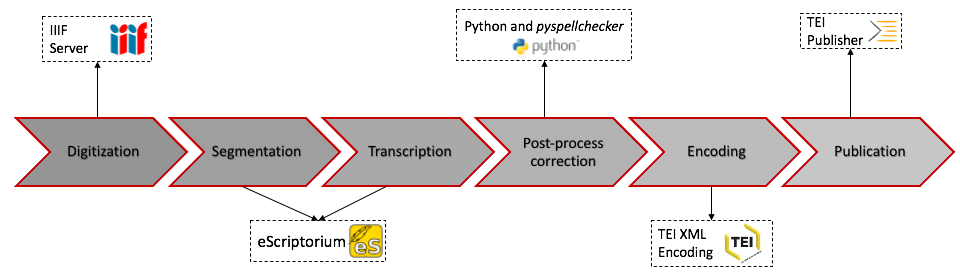
\includegraphics[width=1\linewidth]{2-MAIN//images/pipeline-discholed.png}
    \caption{Chaîne éditoriale de l'application DiScholEd (source~: F. Chiffoleau)}
    \label{fig:pipeline-discholed}
\end{figure}  

La chaîne éditoriale de DiScholEd s'articule actuellement en six étapes. La première étape essentielle est la numérisation. DiScholEd recommande d'héberger les numérisations sur un serveur IIIF\footnote{Pour comprendre le fonctionnement de IIIF~: \texttt{\href{https://iiif.io/get-started/how-iiif-works/}{https://iiif.io/get-started/how-iiif-works/}} (visité le 27/08/2023).}. Le format IIIF est notamment apprécié en raison de son interopérabilité, et du fait qu'il permet la diffusion des images en haute résolution. La transcription d'un document numérisé peut être considérablement accélérée grâce à l'utilisation d'outils de segmentation et de transcription\footnote{DiScholEd recommande l'utilisation d'\textit{eScriptorium}~: \texttt{\href{https://escriptorium.paris.inria.fr/}{https://escriptorium.paris.inria.fr/}} (visité le 27/08/2023).}, basés sur la reconnaissance optique de caractères (OCR) et la reconnaissance d'écritures manuscrites (HTR).

Une fois la transcription vérifiée, il est possible de télécharger un fichier XML de la transcription, prêt à être encodé. Pour cela, il est préférable de suivre les recommandations du standard TEI\footcite{TEIGuidelines}, interopérable et ouvert. L'encodage terminé, le document peut être publié en ligne, sur une plateforme permettant l'affichage de l'encodage sémantique TEI. Notre travail sur les éditions de l'EHRI s'est articulé autour de ces deux dernières étapes de la chaîne éditoriale.  
    \chapter{Les éditions du projet EHRI}
    % Les éditions du projet EHRI

\section{Une nouvelle approche des archives numériques}

\subsection{Une initiative européenne}
L'objectif principal de l'EHRI en tant qu'infrastructure est de promouvoir la recherche sur la Shoah en facilitant l'accès aux documents d'archives, dispersés à travers le monde. Elle doit établir un plan de travail et produire régulièrement des livrables\footnote{Plan de travail et livrables pour EHRI-3~: \texttt{\href{https://www.ehri-project.eu/division-work}{https://www.ehri-project.eu/division-work}}.}.  

Lors de la deuxième phase du projet, nommée EHRI-2 et financée par le programme Horizon 2020, l'EHRI a dédié une partie de son travail au développement d'outils pour l'archivage numérique de documents concernant la Shoah. Cela a pris la forme d'un \textit{Work Package} (WP12) intitulé \enquote{\textit{New Views on Digital Archives}} (\enquote{Nouvelles perspectives sur les archives numériques}). 


\subsection{Développer les éditions numériques sur la Shoah}
L'équipe éditoriale du WP12 a défini les critères qu'elle estime essentiels à une édition numérique sur la Shoah. Parmi ces critères, nous retrouvons une interface claire, dotée d'une bonne fonctionnalité de recherche, l'intégration de leur vocabulaire contrôlé, ainsi que l'affichage des données géographiques sur une carte\footcite[p.~6]{Ehri2018}.  



\section{Les éditions en ligne EHRI}
Chaque édition est une collection\footnote{Nous emploierons les termes \enquote{édition} et \enquote{collection} indistinctement pour faire référence aux éditions en ligne EHRI.} de documents conservés dans les institutions partenaires de l'EHRI. Ce sont des éditions thématiques\footcite{EhriOnlineEditions} reflétant une période ou illustrant un phénomène.



\subsection{BeGrenzte Flucht (2018)}
La première édition publiée par l'EHRI, \enquote{\textit{BeGrenzte Flucht: Die österreichischen Flüchtlinge an der Grenze zur Tschechoslowakei im Krisenjahr 1938}} (\enquote{Fuite entravée~: les réfugié$\cdot$e$\cdot$s autrichien$\cdot$ne$\cdot$s à la frontière tchécoslovaque en 1938\footnote{Les traductions proposées pour les titres des éditions sont les nôtres.}}), a été publiée en 2018. Elle contient cent quatre documents.  

Le nazisme est une idéologie basée sur l'antisémitisme~: la population juive est considérée comme nuisible et sert de bouc-émissaire à la situation de l'Allemagne au sortir de la Première Guerre mondiale. Toutefois, le régime nazi ne semble pas souhaiter l'élimination massive et immédiate des Juifs allemands avant la guerre\footcite[p.~123]{Sallee2018}{}. Sa politique cherche avant tout à exclure et humilier les Juifs, pour les forcer à quitter le territoire\footcite[p.~22]{Bensoussan2020}. Si une grande partie de la population juive quitte l'Allemagne, le \enquote{problème} posé par la \enquote{question juive} a seulement été déplacé et se représente au fur et à mesure que le Reich étend son territoire.  

Le 12 mars 1938, l'Autriche est annexée par l'Allemagne nazie, c'est l'\enquote{\textit{Anschlu\ss{}}}, et la population juive résidant alors en Autriche est contrainte d'émigrer. La Tchécoslovaquie devient l'un des principaux refuge pour les Juif$\cdot$ve$\cdot$s autrichien$\cdot$ne$\cdot$s, mais la politique d'accueil de plus en plus restrictive de la Tchécoslovaquie conduit au blocage complet de la frontière\footnote{À propos de l'édition \enquote{\textit{BeGrenzte Flucht}} (en allemand)~: \texttt{\href{https://begrenzte-flucht.ehri-project.eu/exhibits/show/einleitung}{https://begrenzte-flucht.ehri-project.eu/exhibits/show/einleitung}}.}. L'édition \enquote{\textit{BeGrenzte Flucht}} réunit des documents d'archives principalement tchèques et autrichiens, sous la forme de rapports gouvernementaux, articles de presse et de témoignages direct de victimes et de témoins.  

\begin{figure}[h]
    \centering
    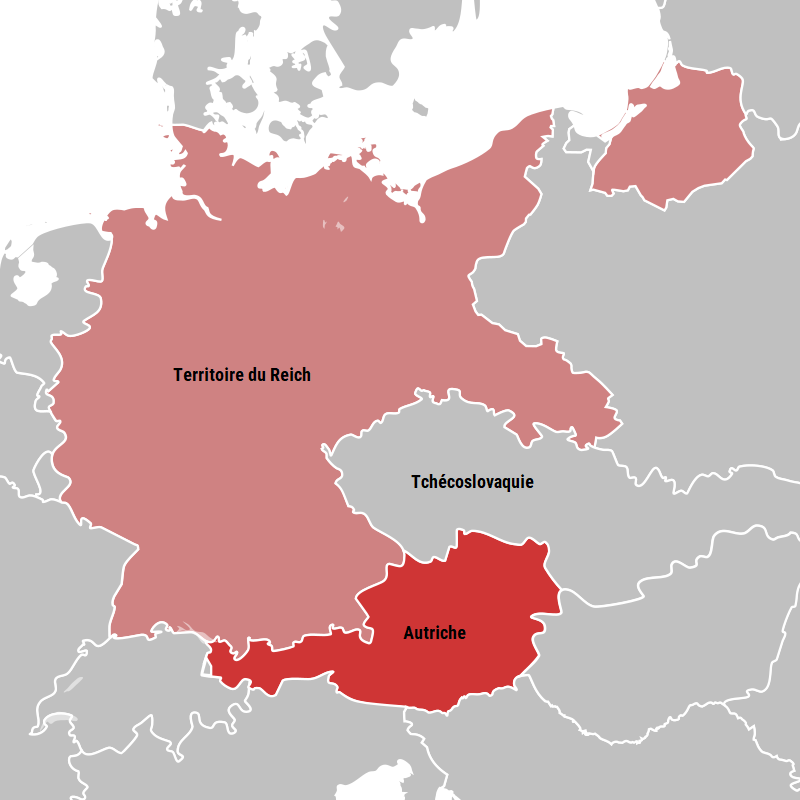
\includegraphics[width=0.8\linewidth]{2-MAIN/images/carte-anschluss.png}
    \caption{Frontières du Reich en mars 1938 (Source~: Wikipédia)}
    \label{fig:anschluss}
\end{figure}

\bigskip
\bigskip
\bigskip
\bigskip
\bigskip

\subsection{Early Holocaust Testimony (2020)}
La deuxième édition publiée par l'EHRI, \enquote{\textit{Early Holocaust Testimony}} (\enquote{Premiers témoignages de la Shoah}), a été publiée en 2020. Elle contient cent dix-neuf documents.  

Il convient tout d'abord de préciser le sens de \enquote{témoignage}. Le TLFi définit le témoignage comme une \enquote{déclaration qui confirme la véracité de ce que l'on a vu, entendu, perçu, vécu\footnote{Entrée complète sur le site du CNRTL~: \texttt{\href{https://www.cnrtl.fr/definition/temoignage}{https://www.cnrtl.fr/definition/temoignage}}}}. La collection \enquote{\textit{Early Holocaust Testimony}} se concentre sur le témoignage écrit, les témoignages oraux ayant été retranscrits. Nous reviendrons ensuite sur le terme \enquote{\textit{early}}, à propos duquel l'équipe éditoriale précise qu'il correspond à tout témoignage de la persécution de la communauté juive depuis le début du régime nazi en 1933 au procès d'Adolf Eichmann à Jérusalem en 1961\footnote{Notre propre traduction, à partir de l'introduction à l'édition (\enquote{\textit{What is an early Holocaust testimony?}})~: \texttt{\href{https://early-testimony.ehri-project.eu/exhibits/show/about/what-is-testimony}{https://early-testimony.ehri-project.eu/exhibits/show/about/what-is-testimony}}.}.


\subsection{Diplomatic Reports (2021)}
La troisième édition publiée par l'EHRI, \enquote{\textit{Diplomatic Reports}} (\enquote{Rapports diplomatiques}), a été publiée en 2021. Elle contient soixante-douze documents venant du Danemark, de l'Italie, du Japon et des États-Unis. De nouveaux rapports provenant de la Hongrie, de la Slovaquie et de la Suède devraient prochainement intégrer la collection.  

La position du$\cdot$de la diplomate est particulière~: il$\cdot$elle est amené$\cdot$e à côtoyer les politicien$\cdot$ne$\cdot$s influent$\cdot$e$\cdot$s du pays où il$\cdot$elle est stationné$\cdot$e, mais doit garder une certaine distance en tant qu'observateur$\cdot$ice. Les informations récoltées doivent être régulièrement communiquées au ministère des Affaires étrangères de leur état d'origine par le biais de rapports.

De nombreux$\cdot$ses diplomates stationné$\cdot$e$\cdot$s en Allemagne nazie ont rapidement compris que les dirigeants nazis ne se contenteraient pas des lois discriminatoires à l'encontre de la population juive. L'étude de ces rapports diplomatiques permet d'aborder la Shoah comme un événement européen auquel de nombreux pays ont activement participé, notamment par la fermeture de leurs frontières\footnote{Voir l'introduction à l'édition, rédigée par Frank Bajohr~: \texttt{\href{https://diplomatic-reports.ehri-project.eu/exhibits/show/about/introduction}{https://diplomatic-reports.ehri-project.eu/exhibits/show/about/introduction}}.}.  


\subsection{Nisko (2023)}
La quatrième édition publiée par l'EHRI, \enquote{\textit{Von Wien ins Nirgendwo: Die Nisko Deportationen 1939}} (\enquote{De Vienne à Nulle Part: les déportations vers Nisko de 1939}), a été publiée en 2023. Elle contient quarante documents.  

En avril 1938, le régime nazi ouvre son agence de l'Office central pour l'émigration juive à Vienne en Autriche\footcite[p.~30]{Bensoussan2020}. Cette agence a pour but d'accélérer l'émigration forcée des Juif$\cdot$ve$\cdot$s autrichien$\cdot$ne$\cdot$s. Au moment de l'annexion de l'Autriche en mars 1938, \enquote{plus de 200~000 personnes étaient considérées comme juives selon les critères des lois raciales de Nuremberg. Les Juifs autrichiens représentaient 40~\%{} des Juifs vivant sur tout le territoire du Grand Reich\footcite[p.~137]{Safrian2007}}. L'agence de Vienne a été libre de \enquote{tester un certain nombre de mesures extrémistes contre les Juifs\footcite[p.~132]{Safrian2007}}, autonome de l'agence principale située à Berlin.  

Le \enquote{Plan Nisko} débute en octobre 1939, un mois seulement après l'invasion de la Pologne. L'idée des dirigeants nazis est de relocaliser la population juive à Lublin et Nisko en Pologne, dans ce qu'ils appellent une \enquote{réserve juive\footcite[p.~34]{Bensoussan2020}}.  

Jusqu'à présent, la recherche sur le \enquote{Plan Nisko} s'est concentrée sur le transport et l'instrumentalisation du train comme premier projet expérimental des futures déportations de masse. La collection \enquote{\textit{Nisko}} se concentre sur la déportation d'environ 1~600 hommes juifs de Vienne les 20 et 26 octobre 1939, en seulement deux trains. Le \enquote{Plan Nisko} est abordé sous l'angle de la vie quotidienne des déportés à travers leur correspondance. Une partie de ces déportés a assuré la construction de la \enquote{réserve juive}, certains ont été capturés et envoyés dans des camps de travail russes, tandis que d'autres encore ont été \enquote{chassés vers l'Est}. Les Nazis appelaient ce phénomène la \enquote{dispersion}.  

Le \enquote{Plan Nisko} se termine en avril 1940 et des rapatriements vers Vienne sont organisés. Toutefois, le sort de ceux qui n'ont pas été rapatriés n'a pu être que partiellement reconstitué\footnote{Voir l'introduction à l'édition \enquote{\textit{Nisko}}, rédigée par Winfried Garscha~: \texttt{\href{https://nisko-transports.ehri-project.eu/exhibits/show/einleitung/nisko-transporte-wien}{https://nisko-transports.ehri-project.eu/exhibits/show/einleitung/nisko-transporte-wien}}.}.  
    \chapter{La diplomatique à l'épreuve du numérique}
    % La diplomatique à l'épreuve du numérique

\section{La diplomatique}

\subsection{En tant que science}
La diplomatique est \enquote{la science qui étudie la tradition, la forme et l'élaboration des actes écrits. Son objet est d'en faire la critique, de juger de leur sincérité, d'apprécier la qualité de leur texte, de dégager des formules tous les éléments du contenu susceptibles d'être utilisés par l'historien, de les dater, enfin de les éditer\footcite[p.~21]{VocArchivistique1997}}. À l'origine, la diplomatique ne servait qu'à analyser les actes médiévaux dans le cadre de contestations judiciaires\footcite[p.~604]{Duranti2003}. Ceci explique pourquoi une partie du vocabulaire utilisé pour décrire les documents n'est pas adaptée à l'analyse de documents contemporains.  


\subsection{L'analyse diplomatique}
L'analyse diplomatique d'un acte est traditionnellement divisée en plusieurs catégories. Les caractéristiques externes\footcite[p.~45-50]{VocArchivistique1997} d'un document concernent sa matérialié, notamment le support utilisé (papyrus, parchemin, papier, etc.). Les caractéristiques internes \footcite[p.~51-68]{VocArchivistique1997} concernent l'écrit lui-même et analyse son contenu.  


\subsection{La diplomatique contemporaine}
Durant la seconde moitié du XX\ieme{} siècle, l'analyse diplomatique a été étendue aux documents administratifs\footcite[p.~604-605]{Duranti2003} et les catégories de documents écrits ont été élargies. On parlera ainsi de \enquote{document dispositif} lorsque l'action juridique dépend de sa mise à l'écrit, de \enquote{document probatoire} lorsque sa mise à l'écrit apporte une preuve à l'action juridique\footcite[p.~22]{VocArchivistique1997}, de \enquote{document à l'appui} quand celui-ci contribue à l'action sans la créer ni la prouver, et enfin de \enquote{document narratif} pour tout document qui ne participe pas à l'action juridique\footcite[p.~605]{Duranti2003}  .



\section{Typologie documentaire des éditions EHRI}
Si l'on se rapporte à la typologie documentaire établie par Luciana Duranti, les éditions EHRI sont composées de documents probatoires, à l'appui et narratifs. Nous distinguons trois types de documents principaux~: les témoignages, les rapports diplomatiques et les articles de presse.  

Chacune des éditions de l'EHRI se concentre sur un aspect de l'histoire de la Shoah. De nombreux documents prennent la forme de témoignages. Au sens de la diplomatique contemporaine, ce sont des documents narratifs décrivant la persécution de la population juive en Europe à partir de 1933. Les témoignages sont de trois natures principales~: les extraits de journaux intimes, la correspondance, et les témoignages oraux. Ces derniers ont été recueillis \textit{a posteriori} et transcrits, notamment les témoignages judiciaires entendus lors des procès des dirigeants nazis après la guerre. Les témoignages ont été rédigés par des Juif$\cdot$ve$\cdot$s eux$\cdot$elles-mêmes ou par des témoins de leur persécution.

Les rapports diplomatiques diffèrent des témoignages dans la mesure où ce sont des documents officiels. Ils prennent parfois la forme d'un document attaché à une lettre, parfois le contenu du rapport se trouve dans un télégramme. Ils témoignent du sort de la population juive, notamment au moment des déportations. Certains rapports sont rédigés sur du papier à lettre officiel, dont il convient d'encoder l'en-tête.  

En plus des témoignages directs, les collections contiennent également de nombreux articles parus dans la presse. Seul le texte de l'article est encodé, même lorsque toute une page du journal est numérisée.  



\section{Le standard TEI pour l'encodage des documents}

\subsection{Un standard ouvert et interopérable}
La TEI est un standard qui a été développé \enquote{par la communauté scientifique, pour son propre usage\footcite{Burnard2015}}. Elle s'appuie sur le métalangage XML et permet un encodage sémantique du texte. Contrairement au traitement de texte, qui s'attache plutôt à l'apparence du texte, la TEI permet par exemple de différencier sémantiquement des homonymes, de sorte que lors de la construction d'un index les occurrences ne seront pas confondues.  

En outre, la TEI est un standard interopérable, et un texte encodé suivant ses recommandations sera toujours lisible. Elle est détachée de tout logiciel et des mises à jours dont celui-ci aurait besoin, ou de son obsolescence. L'encodage TEI est lisible par l'humain.  


\subsection{Diplomatique et TEI}
Les documents encodés en TEI ont une structure initiale identique~: le \texttt{<teiHeader>} et le \texttt{<text>}. Le \texttt{<teiHeader>} regroupe les métadonnées concernant le document. Cette section a une structure minimale obligatoire mais peut être étendue au besoin. Dans notre processus de création du nouveau modèle d'encodage pour les éditions en ligne de l'EHRI, nous avons considérablement précisé les champs contenus dans le \texttt{<teiHeader>} (Annexe \ref{Metadonnees}). Le \texttt{<text>} contient l'encodage de la partie textuelle du document. Il contient un élément \texttt{<body>} qui peut être divisé en sections avec des éléments \texttt{<div>} (\enquote{\textit{ext division}}) selon la structure du texte.  

La diplomatique, comme toutes les sciences, dispose d'un vocabulaire spécifique. La notion de \enquote{protocole}, par exemple, n'est pas représentée en tant que telle au sein de la TEI\footcite[p.~185]{Clavaud2015}. Toutefois, un encodage rigoureux du texte et des métadonnées permet d'identifier toutes les informations qui seraient regroupées sous l'appellation \enquote{protocole} (initial ou final) dans une analyse diplomatique.

    % Partie 2
    \part{Modèle d'encodage}
    \chapter{Encodage des éditions EHRI}
    % Analyse des pratiques d'encodage des éditions en ligne EHRI

\section{Analyse des pratiques d'encodage}
Avec la publication de plusieurs éditions thématiques, l'équipe d'éditoriale de l'EHRI a pu expérimenter l'utilisation de la TEI et adapter sa pratique. Notre travail a donc débuté par l'observation des pratiques d'encodage des précédentes éditions.  

\subsection{Extraction de l'information}
Le corpus à analyser était composé des quatre éditions, soit un total de trois cent trente-cinq documents. À l'aide d'un \textit{script} Python, nous avons pu extraire toutes les occurrences des balises et attributs utilisés par collection. Nous avons ensuite arrangé les résultats dans un tableau récapitulatif (Annexe \ref{Tableau}).  

\begin{figure}[h]
    \centering
    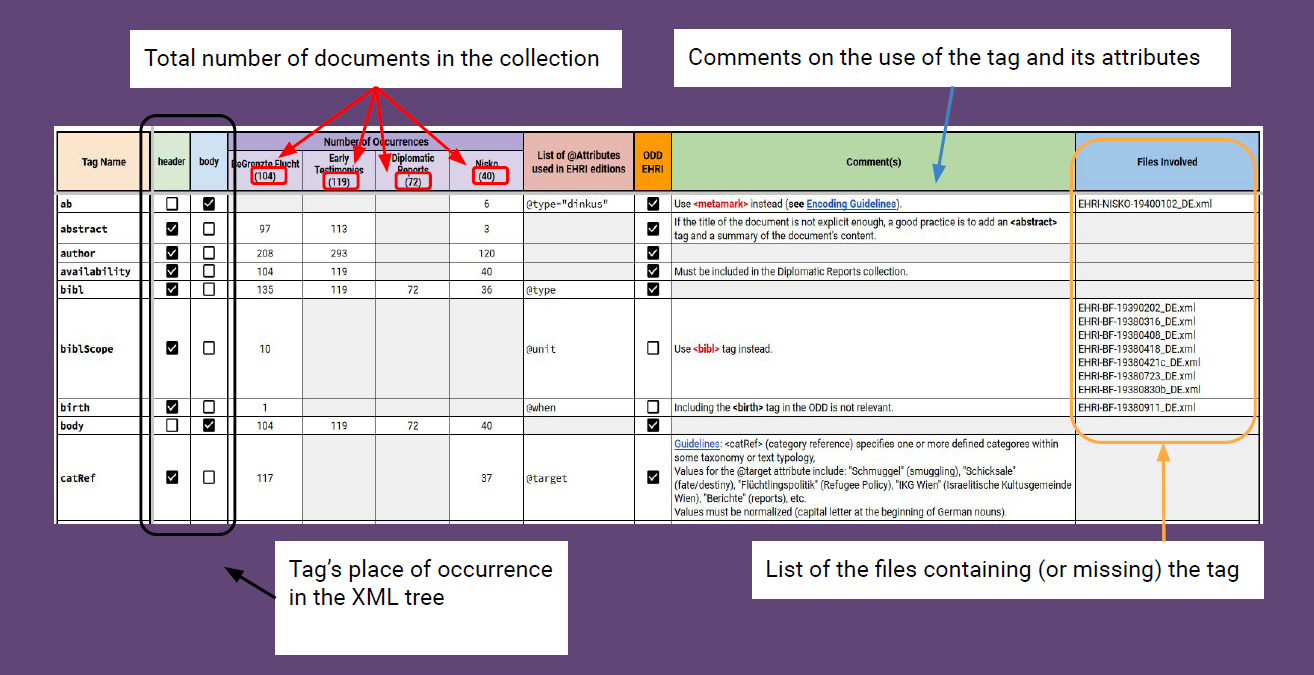
\includegraphics[width=0.95\linewidth]{2-MAIN//images/tableau-fonctionnement.png}
    \caption{Fonctionnement du tableau récapitulatif de l'encodage des éditions EHRI}
    \label{fig:tableau-recap}
\end{figure}  

Les balises sont classées par ordre alphabétique, et une case à cocher permet de voir si la balise se trouve dans le \texttt{<teiHeader>} et/ou dans le \texttt{<body>}. Chaque collection dispose ensuite de sa propre colonne, indiquant pour chaque balise son nombre d'occurrences. Nous avons ensuite établi, pour chaque balise, une liste de tous ses attributs utilisés dans l'encodage EHRI.


\subsection{Évaluation du choix des balises et attributs}
Une fois le tableau récapitulatif en partie rempli, nous avons pu procéder à une analyse plus approfondie de l'encodage. En fonction du contexte, nous avons ajouté des commentaires sur l'utilisation de certaines balises~; une précision sur l'usage recommandé par les \textit{TEI Guidelines} ou une suggestion d'amélioration, par exemple.  

Le tableau a été rendu le plus complet possible grâce à la rédaction d'un \textit{script}, en Python, permettant de rechercher des informations précises dans le corpus (extrait du code en Annexe \ref{Script}). Le nombre d'occurrences de certaines balises a révélé des doublons, à l'instar de la balise \texttt{<creation>}, apparaissant parfois deux fois au sein d'un même fichier. Or, la création d'un document ne peut avoir qu'une seule occurrence. Ce \textit{script} nous a permis de remplir la dernière colonne du tableau, \enquote{\textit{Files Involved}}, pour que les éditeur$\cdot$ice$\cdot$s puissent corriger ce type d'erreurs.



\section{Identification des améliorations possibles}
Le tableau complet donne une bonne vue d'ensemble de l'encodage des éditions EHRI, et notamment de leur évolution. Nous avons identifié deux pistes d'améliorations significatives~: une meilleure conformité aux recommandations de la TEI et l'uniformisation des éditions déjà publiées.  

\subsection{Amélioration de la conformité}
Pour être conforme au standard TEI, un fichier XML doit être bien formé, c'est-à-dire rédigé avec une syntaxe correcte. Le fichier XML doit également être valide. Pour cela, il faut que l'encodage respecte les règles du schéma qui lui a été associé. Enfin, le projet d'encodage doit être renseigné de façon exhaustive dans une ODD\footnote{Nous aborderons la notion d'ODD dans le chapitre suivant.} (\enquote{\textit{One Document Does-it all}}), elle aussi conforme.  

Parmi les bonnes pratiques que nous recommandons dans le traitement d'un corpus comme celui des éditions EHRI, il y a tout d'abord la question de l'identifiant du fichier. Les fichiers EHRI portent tous un identifiant unique basé sur une même structure~: \enquote{\texttt{EHRI-<collection>-YYYYMMDD\_{}<langue>}} (par exemple, \enquote{\texttt{EHRI-BF-19380315\_{}DE}}). Cet identifiant doit être la valeur de l'attribut \texttt{@xml:id} qui se trouve dans la balise ouvrante de l'élément racine \texttt{<TEI>}.  

Le seconde recommandation qui nous paraît particulièrement importante est la structuration du contenu à l'intérieur de la balise \texttt{<body>}. Pour assurer un bon affichage du contenu et éviter la multiplication inutile de fichiers, nous proposons d'encoder la transcription du fac-similé et ses traductions au sein d'un même fichier. Il y aurait donc au moins une division \texttt{<div>} de premier niveau, complétée par un attribut \texttt{@type} dont la valeur serait \texttt{"transcription"} ou \texttt{"translation"}. Dans le cas des traductions, l'attribut \texttt{@xml:lang} apporterait une précision sur la langue de la traduction contenue dans la division.


\subsection{Uniformisation des édition}

\subsubsection{Utilisation de l'anglais}
La nature européenne du projet EHRI implique que les différents acteurs ne parlent pas tous la même langue. La langue la plus communément parlée parmi les éditeur$\cdot$ice$\cdot$s et le public des éditions est l'anglais. Il nous paraît donc logique de normaliser l'utilisation de l'anglais comme langue d'encodage des métadonnées et de la valeur des attributs. Cela permet à quiconque accédant aux fichiers XML d'en comprendre l'encodage. Nous avons ainsi parfois été confronté$\cdot$e à des valeurs d'attributs en allemand. Le problème posé par l'utilisation de l'allemand pour préciser la valeur des attributs est le risque d'une perte sémantique lors de sa traduction dans une autre langue. Or, les valeurs d'attributs proposées par les \textit{TEI Guidelines} dans leur documentation d'éléments sont toujours en anglais, ce qui facilite le travail d'encodage et la réutilisation du schéma produit pour l'édition.

\subsubsection{Standardisation de la valeur de certains attributs}
Il est essentiel que les valeurs des attributs soient uniformes. Pour certains attributs, il existe des normes que l'on peut choisir d'appliquer. Par exemple, il existe une norme d'encodage concernant le format des dates~: l'utilisation de l'attribut \texttt{@when-iso} sera privilégié si la date est au format \enquote{\texttt{YYYY-MM-DD}} (norme ISO 8601\footnote{Récapitulatif de la norme ISO 8601 sur Wikipédia~: \texttt{\href{https://fr.wikipedia.org/wiki/ISO_8601}{https://fr.wikipedia.org/wiki/ISO\_{}8601}} (visité le 03/09/2023).}), sinon on lui préférera l'attribut \texttt{@when}. Cela est d'autant plus important qu'une date incomplète avec un attribut \texttt{@when-iso} causera un bug d'affichage, et qu'une date complète avec un attribut \texttt{@when} ne s'affichera pas correctement. Il n'existe, en revanche, pas de normes concernant l'attribut \texttt{@type}, ses valeurs possibles étant aussi variées que la diversité des éléments auquel il peut être associé.  

L'importance de la valeur de l'attribut \texttt{@xml:lang} peut paraître abstraite. En général, et même s'il est possible d'écrire le nom de la langue en toutes lettres, nous utilisons un code pour donner la valeur de l'attribut de langue. Or, ce code doit s'inscrire dans un système établi~: c'est le rôle des normes. Prenons l'exemple de la langue allemande~: \enquote{Allemand} en français, \enquote{\textit{German}} en anglais, et \enquote{\textit{Deutsch}} en allemand. Sans système pré-établi, l'éditeur$\cdot$ice sera naturellement tenté$\cdot$e d'utiliser un code parlant pour sa propre langue. Nous obtiendrions donc les possibilités suivantes~: \enquote{\texttt{"all"}}, \enquote{\texttt{"ger"}} et \enquote{\texttt{"deu"}} respectivement. Le problème devient évident. Le choix ne peut pas revenir à l'éditeur$\cdot$ice de déterminer lui$\cdot$elle-même des codes à utiliser. Il existe en outre des préférences, qui ne regardent que les traducteur$\cdot$ice$\cdot$s, concernant le choix de traduire certains termes ou de les laisser apparaître dans leur langue originale. Ce problème s'applique également ici.  

Plusieurs systèmes existent. La norme ISO 639\footnote{Récapitulatif de la norme ISO 639 sur Wikipédia~: \texttt{\href{https://fr.wikipedia.org/wiki/ISO_639}{https://fr.wikipedia.org/wiki/ISO\_{}639}} (visité le 03/09/2023).} définit des codes pour les langues à deux ou trois caractères (ISO 639-1 ou ISO 639-2). Le problème posé par cette norme est qu'elle ne tranche pas entre l'utilisation de deux ou trois caractères, ce qui peut conduire à une certaine confusion. Nous avons donc opté pour le registre de codes établi par l'Iana\footnote{\enquote{\textit{Iana Language Subtag Registry}}~: \texttt{\href{https://www.iana.org/assignments/language-subtag-registry/language-subtag-registry}{https://www.iana.org/assignments/language-subtag- registry/language-subtag-registry}}.}. Celui-ci a l'avantage de ne proposer qu'une norme, précise et très régulièrement mise à jour. 
    \chapter{Définition du nouveau modèle d’encodage}
    % Définition du nouveau modèle d'encodage

\section{\textit{One Document Does-it-all}}

Une ODD (\enquote{\textit{One Document Does-it-all}}) est un fichier XML encodé en TEI dont l'objectif est double. Elle permet de documenter le projet éditorial, en prose, mais également de créer des règles de validation. Ces dernières seront exportées dans un schéma RelaxNG, qui sera appliqué aux fichiers pour guider et valider leur encodage.

Il existe trois principales façons de générer une ODD~: l'utilisation de l'interface ROMA\footnote{ROMA~: \texttt{\href{https://roma.tei-c.org/}{https://roma.tei-c.org/}}.} créée par le TEI Consortium, l'utilisation de la feuille de style XSL \enquote{\textit{Oddbyexample}} à partir d'un encodage préexistant, ou la rédaction manuelle de l'ODD à partir de rien. Nous avons rapidement éliminé les deux dernières options et choisi de générer la base de notre ODD avec ROMA. En effet, la création de l'ODD manuellement aurait été trop chronophage, et la génération à partir de \enquote{\textit{Oddbyexample}} aurait nécessité de corriger les fichiers EHRI en amont~; or la répartition des balises est parfois inégale au sein des trois cent trente-cinq fichiers.  

La solution la plus optimale dans notre cas a donc été de travailler avec ROMA en partant du schéma le plus large~: \enquote{\textit{TEI All}}. L'application directe de ce schéma serait tout à fait inutile, puisqu'il contient tous les éléments de la TEI, alors que le projet n'en utilise qu'une partie. Il existe d'autres schémas spécifiques mais pour être pertinent, le schéma doit correspondre le plus possible aux caractéristiques du projet.  

La customisation de l'ODD avec ROMA se présente sous la forme d'une liste des éléments de la TEI accompagnés d'une brève présentation et d'une case à cocher. Les éléments peuvent être classés par ordre alphabétique ou par module. Dans leur rapport, les éditeur$\cdot$ice$\cdot$s de l'EHRI ont souligné l'importance du module \texttt{namesdates} dans leur encodage\footcite{Ehri2018}. Pour créer le modèle le plus pertinent possible, nous nous sommes attaché$\cdot$e à consulter la documentation de tous les éléments qui nous paraissaient pertinents, en particulier concernant l'encodage des métadonnées dans le \texttt{<teiHeader>}. Une fois la base de l'ODD générée, il convient de rédiger consciencieusement la documentation et de créer des règles de validation fonctionnelles.  



\section{Rédaction de la documentation}
Nous avons divisé la rédaction de la documentation de l'ODD en trois sections~: les règles fondamentales, l'encodage du \texttt{<teiHeader>} et l'encodage du \texttt{<body>}. L'idée de la documentation de l'ODD est de s'affranchir de la seule consultation des \textit{TEI Guidelines} et d'illustrer l'usage que nous en faisons dans le cadre du projet, notamment grâce à des exemples tirés de notre propre corpus.  

La création du tableau récapitulatif (Annexe \ref{Tableau}), et les commentaires que nous y avons inclus, nous a permis de dégager certaines pratiques que les éditions en ligne de l'EHRI auraient tout intérêt à adopter pour assurer la conformité et l'uniformité de leur encodage. Ce sont les recommandations d'uniformisation que nous évoquions dans le chapitre précédent.  

En analysant l'encodage des collections, nous avons pu adapter la structure du \texttt{<teiHeader>} (Annexe \ref{Metadonnees}). Cette partie de la documentation est particulièrement longue, mais il nous paraissait essentiel d'insister dessus dans la mesure où les membres de l'équipe éditoriale de l'EHRI sont nombreux et que la composition de l'équipe peut être amenée à changer au fil des années. C'est cette partie qui a nécessité le plus de clarifications, dans la mesure où nombre d'éléments figuraient déjà dans l'encodage des métadonnées, mais leur utilisation a été réadaptée dans notre nouveau modèle.  

Enfin, nos recommandations pour l'encodage du \texttt{<body>} ont été guidées par la volonté de transcrire la structure du fac-similé le plus fidèlement possible. Nous avons donc insisté sur l'utilisation des balises \texttt{<pb/>} (\enquote{\textit{page beginning}}) et \texttt{<lb/>} (\enquote{\textit{line beginning}}) pour que l'affichage lors de la publication soit le plus proche possible du fac-similé. Nous avons également affiné l'encodage en introduisant les éléments \texttt{<opener>} et \texttt{<closer>}, contenant tous les deux les informations relatives aux en-têtes des documents et aux éléments de salutations.



\section{Création du schéma de validation}
Les règles du schéma de validation sont contenues dans un élément \texttt{<schemaSpec>} (\enquote{\textit{schema specification}}).  

\subsection{Déclaration des modules}
Les éléments de la TEI sont classés en modules. Quatre d'entre eux sont obligatoires et communs à tous les encodages~: \texttt{tei}, \texttt{header}, \texttt{core} et \texttt{textstructure}. Les modules sont déclarés à l'aide de l'élément \texttt{<moduleRef>} (\enquote{\textit{module reference}}). Le module déclaré est précisé par la valeur de l'attribut \texttt{@key}.  

Il existe ensuite deux façons de déclarer les éléments de chaque module acceptés par le schéma de validation~: l'attribut \texttt{@include} déclare les éléments autorisés, tandis que l'attribut \texttt{@except} déclare les éléments non-autorisés. Dans un souci de légèreté et de lisibilité, il est généralement conseillé de choisir le mode de déclaration en fonction du nombre d'éléments à déclarer. Ainsi, si l'on souhaite utiliser tous les éléments du module \texttt{namesdates} sauf les éléments \texttt{<age>} et \texttt{<birth>}, par exemple, il est conseillé de les exclure avec l'attribut \texttt{@except}. Toutefois, nous avons choisi, dans notre modèle, de n'utiliser que l'attribut \texttt{@include}, que nous estimons plus parlant pour des personnes qui ne seraient pas familières de la TEI.


\subsection{Règles de validation des éléments}
La personnalisation des règles de validation des éléments se fait grâce à l'élément \texttt{<elementSpec>} (\enquote{\textit{element specification}}), qui contient les informations sur la structure et le contenu possible de l'élément. Il n'est pas nécessaire de déclarer ici les éléments qui restent inchangés. Nous avons établi pour les éditions EHRI des règles de validation mettant en place les recommandations exprimées dans la partie documentation. Il s'agissait le plus souvent de déclarer le caractère recommandé (\texttt{"rec"} pour \enquote{\textit{recommended}}) ou obligatoire (\texttt{"req"} pour \enquote{\textit{required}}) d'un attribut, et éventuellement de définir une liste semi-ouverte de valeurs (comme pour l'attribut \texttt{@xml:lang}).


\subsection{Déclaration des classes d'attributs}
Les attributs sont regroupés en classes. Par exemple, la plupart des attributs précisant l'affichage souhaité de l'encodage appartiennent à la classe \texttt{att.global.rendition}. Certains attributs, comme \texttt{@type}, appartiennent à plusieurs classes d'attributs, et chaque élément prend en charge certaines classes définies. La déclaration des classes d'attributs permet donc de limiter l'usage des attributs à celui que l'on souhaite en faire dans le cadre du projet.
    \chapter{Semi-automatisation du modèle}
    % Semi-automatisation du modèle

\section{Automatisation et semi-automatisation}
La mission de l'Inria sur le projet EHRI est de proposer un soutien technique, que les éditeur$\cdot$ice$\cdot$s sont libres d'utiliser ou non. Si certaines tâches peuvent être automatisées, à l'aide de \textit{scripts} Python par exemple, leur utilisation n'est pas forcément à la portée de tout le monde et les éditeur$\cdot$ice$\cdot$s pourraient préférer une solution plus accessible.  

La créatrice de l'application DiScholEd, Floriane Chiffoleau, a rédigé une série de \textit{scripts} d'automatisation\footnote{Voir le dépôt GitHub du projet DAHN~: \texttt{\href{https://github.com/FloChiff/DAHNProject}{https://github.com/FloChiff/DAHNProject}}.} de plusieurs étapes de la chaîne éditoriale, notamment concernant l'encodage des métadonnées et la gestion des entités nommées. L'adaptation de ces \textit{scripts} aux collections de l'EHRI fait partie des prochaines étapes du travail sur le projet.  

Il n'est actuellement pas envisageable d'automatiser tout ou partie de la chaîne éditoriale des éditions EHRI. C'est pourquoi nous avons opté pour une semi-automatisation du processus d'encodage en proposant aux éditeur$\cdot$ice$\cdot$s des \textit{templates} (\enquote{modèles\footnote{Nous utiliserons le terme anglais \enquote{\textit{template}} afin d'établir une distinction avec la notion de \enquote{modèle d'encodage}, qui fait référence à l'ODD et aux règles mises en place.}}) pour l'encodage de certaines parties des fichiers.



\section{Création des \textit{templates} d'encodage}
Nous avons créé deux sortes de \textit{templates} d'encodage. Le premier, et le plus conséquent, concerne l'encodage des métadonnées (Annexe \ref{Metadonnees})~; le second concerne les entrées des index. Il existe trois index aux éditions EHRI~: un index de lieux, un index de personnes et un index des organisations. Nous avons créé un quatrième \textit{template} pour un \enquote{index de termes}. Actuellement, des renvois sont faits vers le vocabulaire contrôlé disponible sur le portail de l'EHRI\footnote{Vocabulaire sur le portail de l'EHRI~: \texttt{\href{https://portal.ehri-project.eu/vocabularies}{https://portal.ehri-project.eu/vocabularies}}.}.  

L'idée derrière la création de ces \textit{templates} est de permettre aux éditeur$\cdot$ice$\cdot$s de gagner du temps en leur proposant une structure à compléter. Cela permet de s'assurer que le plus de champs seront renseignés, et d'éviter des confusions entre différents éléments.  

\begin{figure}[h]
    \centering
    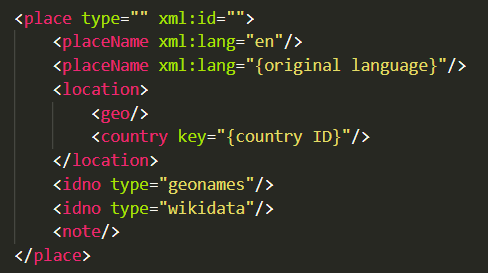
\includegraphics[width=0.7\linewidth]{2-MAIN/images/index.png}
    \caption{\textit{Template} d'une entrée dans l'index de lieux}
    \label{fig:index}
\end{figure}

La Figure \ref{fig:index} représente le \textit{template} d'entrée dans l'index de lieux. Il est bien sûr possible d'ajouter des éléments \texttt{<placeName>} pour chaque langue si le nom du lieu a été traduit, tout comme il est possible de supprimer l'élément \texttt{<placeName xml:lang="en">} si le nom du lieu est typique de sa langue originale et n'a jamais été traduit. L'objectif n'est pas de proposer une traduction, mais de la renseigner, si elle existe, pour faciliter la recherche d'information. Nous estimons qu'il est important d'établir un lien entre les index des éditions et les bases de données publiques largement utilisées comme Geonames\footnote{Geonames~: \texttt{\href{https://www.geonames.org/}{https://www.geonames.org/}}.} et Wikidata\footnote{Wikidata~: \texttt{\href{https://www.wikidata.org/wiki/Wikidata:Main_Page}{https://www.wikidata.org/}}.}, lorsque cela est possible.

    % Partie 3
    \part{Publication et valorisation}
    \chapter{Choix de l'outil de publication}
    % Choix de l'outil de mise en ligne

Nous avons mentionné deux formes que peuvent prendre les éditions numériques~: un \textit{ebook} ou un site web. Selon la méthode de publication choisie, des connaissances en programmation et en développement web peuvent s'avérer nécessaires. Nous en verrons trois~: la création d'un site à partir des fichiers XML grâce à une transformation XSLT, la création d'une application web, et l'utilisation d'une plateforme de publication.    


\section{Méthodes de publication}

\subsection{Transformation XSLT vers HTML}
XSLT est le langage de transformation de l'environnement XML. Un fichier XSL est une feuille de style qui contient des \enquote{\textit{templates\footcite[chapitre 8]{HaroldMeans2002}}}. Cette feuille de style permet de transformer un fichier XML. Le fichier de sortie peut être un autre fichier XML ou dans un autre format~; dans notre cas, il s'agirait d'un fichier HTML.  

Pour opérer une transformation, il faut indiquer au processeur XSL la position de l'élément à transformer grâce à une expression XPath. Pour chaque type de page web que nous souhaitons créer, il faudra créer un \textit{template} contenant les règles de transformation. Par exemple, dans le cas des éditions EHRI, il faudrait créer des \textit{templates} pour la page d'accueil générale des éditions, pour les collection, et pour l'affichage du document. L'élément \texttt{<xsl:template>} contient donc le code HTML que l'on souhaite voir apparaître dans le fichier de sortie, où chaque élément qui dépend du fichier d'entrée (son titre, par exemple) est identifié par son expression XPath. Cela permet de contrôler le niveau de l'arbre XML où sont appliquées les transformations\footcite[chapitre 8]{HaroldMeans2002}.


\subsection{Création d'une application web}
La création d'une application web requiert des connaissances en programmation. Plusieurs langages sont disponibles pour le développement d'une application web~: Python, JavaScript, PHP, Ruby, etc. Nous nous concentrerons sur le langage Python.  

Comme de nombreux langages de programmation, Python dispose de \textit{frameworks}. Un \textit{framework} permet de développer une application grâce à des outils intégrés. Par exemple, le \textit{framework} Flask \footnote{Documentation de Flask (version 2.3)~: \texttt{\href{https://flask.palletsproject.com/en/2.3.x/}{https://flask.palletsprojects.com/en/2.3.x/}}.} permet de créer des \enquote{routes} (URL) qui afficheront la page web associée au \textit{template} HTML. Cette méthode suppose la création d'une base de données dans laquelle Flask ira chercher les informations pour créer l'affichage du site, ce qui nécessite des compétences supplémentaires en gestion de bases de données.


\subsection{Utilisation d'une plateforme de publication}
Enfin, la troisième méthode, qui est sûrement la plus populaire, est le recours à un système de gestion de contenu (CMS). Cette méthode consiste en l'utilisation d'outils permettant aux chercheur$\cdot$euse$\cdot$s de publier leur édition numérique sans devenir développeur$\cdot$euse$\cdot$s. Nous n'évoquerons dans ce mémoire que deux solutions~: Omeka et TEI Publisher.   



\section{Les éditions EHRI et le logiciel Omeka}
Pour la publication de leurs éditions en ligne, l'EHRI a opté en 2018 pour l'utilisation du logiciel \textit{open source} Omeka\footnote{Omeka~: \texttt{\href{https://omeka.org/}{https://omeka.org/}}.}. C'est un CMS, \enquote{dédié à l'organisation, à l'exposition, à la mise en ligne de données iconographiques, avec leur métadonnées, qui permet d'en faire très facilement une publication sur le Web\footcite[p.~81]{BoulaireCarabelli2017}}. Il est également précisé qu'Omeka est \enquote{spécialisé dans l'édition de collections muséales, de bibliothèques numériques et d'éditions savantes en ligne\footcite[p.~115]{IdmhandRiffardWalter2017}.} Il existe deux versions disponibles d'Omeka avec des fonctionnalités différentes~: \enquote{Omeka Classic}, que nous aborderons dans ce mémoire, et \enquote{Omeka S}, davantage orienté vers le web sémantique\footnote{Pour en savoir plus sur Omeka~: \texttt{\href{https://omeka.org/about/project/}{https://omeka.org/about/project/}}.}.

\subsection{Fonctionnement d'Omeka Classic}
Omeka permet la gestion, la valorisation et la diffusion d'importantes collections numérisées\footcite[p.1]{Leblanc2020}. C'est un outil pensé pour la réalisation d'édition \enquote{numérisées\footcite[p.~27]{Sahle2016}} (\enquote{\textit{digitized edition}}) et non numériques (\enquote{\textit{digital edition}})\footcite[p.~2]{Leblanc2020}.  

Deux utilisations se distinguent de l'utilisation d'Omeka. Le logiciel permet de \enquote{représenter de manière structurée et normalisée des connaissances sur des documents\footcite[diapo 7]{Daussin2019}}, mais également de \enquote{construire des parcours raisonnés à l’aide de pages web dans une sélection ou une collection de
documents\footcite[diapo 7]{Daussin2019}}, et ce à des fins de partage ou de conservation.  

Un \enquote{contenu Omeka\footcite[diapo 8]{Daussin2019}} est composé d'un document et de ses métadonnées~; le document lui-même pouvant être composé de plusieurs fichiers. Les métadonnées sont signalées à l'aide du standard Dublin Core et décrivent le contenu (titre, sujet, description, source,  langue, relation et couverture), la propriété intellectuelle (créateur, contributeur, éditeur et gestion des droits) et l'instanciation (date, type, format, identifiant de la ressource)\footnote{Pour plus d'informations sur le standard Dublin Core~: \texttt{\href{https://www.bnf.fr/fr/dublin-core}{https://www.bnf.fr/fr/dublin-core}} (visité le 02/09/2023).}.


\subsection{Limites posées par le recours à Omeka}
Pour les chercheur$\cdot$euse$\cdot$s souhaitant publier proprement leur édition sans avoir à apprendre la programmation, l'utilisation d'Omeka présente de nombreux avantages. Le logiciel permet notamment de gérer un volume conséquent de données et de valoriser son contenu par la création d'\enquote{expositions virtuelles, \textins{de} cartes et \textins{de} frises chronologiques\footcite[p.~18-19]{Leblanc2020}}.  

Pourtant, et spécifiquement pour la création d'éditions numériques, Omeka présente un inconvénient non négligeable~: le logiciel n'est pas conçu pour traiter des documents encodés en TEI. Ce sont les équipes des projets travaillant sur Omeka qui ont développé des modules (\textit{plug-ins}) pour permettre le traitement et l'affichage de ces éditions\footcite[p.~4]{Leblanc2020}, alors que le standard TEI est le plus utilisé par l'édition scientifique numérique.  

\bigskip
\bigskip
\bigskip
\bigskip
À titre d'exemple, l'équipe éditoriale du WP12 de l'EHRI a dû mettre au point une correspondance entre certains éléments du \texttt{<teiHeader>} et les champs du Dublin Core\footcite[p.~7-9]{Ehri2018} pour pouvoir travailler avec Omeka\footcite[p.~9]{Leblanc2020}. Cette opération s'apparente donc à une sorte de \enquote{bricolage numérique\footcite[p.~96]{BoulaireCarabelli2017}} et nécessiterait systématiquement la présence d'un$\cdot$e ingénieur$\cdot$e dans l'équipe du projet, ce qui est loin d'être le cas en Sciences Humaines et Sociales\footcite[p.~98]{BoulaireCarabelli2017}.  

Enfin, les modules développés par les équipe de projets pour ajouter des fonctionnalités à Omeka en fonction de leurs besoins peuvent ne plus être compatibles avec le logiciel au fur et à mesure de ses mises à jour. En plus du lourd travail de développement nécessaire à la création d'un module, celui-ci doit être maintenu et la compatibilité avec la version courante d'Omeka doit être assurée\footcite[p.~16]{Leblanc2020}. Or, ce sont des missions que les chercheur$\cdot$euse$\cdot$s ne peuvent pas assurer eux$\cdot$elles-mêmes, d'une part parce que c'est une activité très chronophage, et d'autre part parce que cela relève d'un domaine qui n'est pas le leur.  



\section{Une autre alternative~: TEI Publisher}

\subsection{Fonctionnement de TEI Publisher}
TEI Publisher se présente comme un outil permettant aux chercheur$\cdot$euse$\cdot$s et aux éditeur$\cdot$ice$\cdot$s de publier leurs éditions numériques sans apprendre la programmation, tout en laissant une place importante à la personnalisation. Son objectif est de fournir à ses utilisateur$\cdot$ice$\cdot$s une structure fonctionnelle, bien pensée et personnalisable\footnote{Documentation TEI Publisher~: \texttt{\href{https://teipublisher.com/exist/apps/tei-publisher/doc/documentation.xml?odd=docbook&view=div}{https://teipublisher.com/exist/apps/tei-publisher/doc/ documentation.xml?odd=docbook\&view=div}} (visité le 02/09/2023).}.  

Une fois installée, la plateforme est dotée d'une \enquote{aire de jeu\footnote{Disponible depuis la page d'accueil de la plateforme~: \texttt{\href{https://teipublisher.com/exist/apps/tei-publisher/index.html?query=&collection=playground&sort=title&field=text&start=1}{https://teipublisher.com/exist/apps/ tei-publisher/index.html?query=\&collection=playground\&sort=title\&field=text\&start=1}}.}} pour comprendre le fonctionnement de l'outil. L'affichage du document dépend des réglages de l'ODD\footnote{À ne pas confondre avec la documentation de l'encodage du projet d'édition. L'ODD de TEI Publisher permet de gérer l'affichage du document.} choisie. TEI Publisher prend en charge toutes sortes de documents en entrée, et pas seulement des documents encodés en TEI\footcite{Chiffoleau2020}{}, bien qu'il s'agisse du standard recommandé.  

\bigskip
La personnalisation de son application s'effectue à l'aide de modules appelés \enquote{\textit{web components\footnote{Documentation sur les modules~: \texttt{\href{https://cdn.tei-publisher.com/@2.12.6/dist/api.html}{https://cdn.tei-publisher.com/@2.12.6/dist/api.html}}.}}}.


\subsection{Pourquoi choisir TEI Publisher}
TEI Publisher est un outil \textit{open source} et bien documenté. Sa communauté est très active et la plateforme est mise à jour régulièrement\footnote{La dernière version de TEI Publisher (8.0) a été publiée le 28 mars 2023~: \texttt{\href{https://www.e-editiones.org/posts/tei-publisher-8/}{https://www.e-editiones.org/posts/tei-publisher-8/}}.}. De nombreux projets d'éditions numériques utilisent désormais TEI Publisher, et les nouvelles fonctionnalités développées pour un projet en particulier sont mises à disposition des autres utilisateur$\cdot$ice$\cdot$s. C'est un avantage non négligeable par rapport au logiciel Omeka.  

La capacité de l'outil à prendre en charge des formats comme le DOCX\footnote{Format du traitement de texte Microsoft Word.} est un avantage pour les utilisateur$\cdot$ice$\cdot$s qui n'auraient que peu, voie aucunes, compétences en encodage TEI. À titre d'exemple, les éditeurs du WP12 de l'EHRI encodent leurs documents à l'aide d'un traitement de texte simple avec des liens hypertextes. Le fichier est ensuite transformé en XML-TEI avec l'outil \enquote{Odette\footnote{Odette~: \texttt{\href{https://obvil.huma-num.fr/odette/}{https://obvil.huma-num.fr/odette/}}.}}. En utilisant TEI Publisher, cette étape deviendrait superflue et le travail s'en trouverait accéléré.  

En outre, il nous semble important de souligner que TEI Publisher propose un affichage horizontal des documents (Figure \ref{fig:doc-teipublisher}). Les éditions en ligne de l'EHRI disposent d'un affichage vertical (Figure \ref{fig:ehri-omeka}) centré sur la transcription. Or, cet affichage ne nous semble pas des plus pratiques, notamment en raison du peu d'importance qui est accordé au fac-similé.  

\begin{figure}[!h]
    \centering
    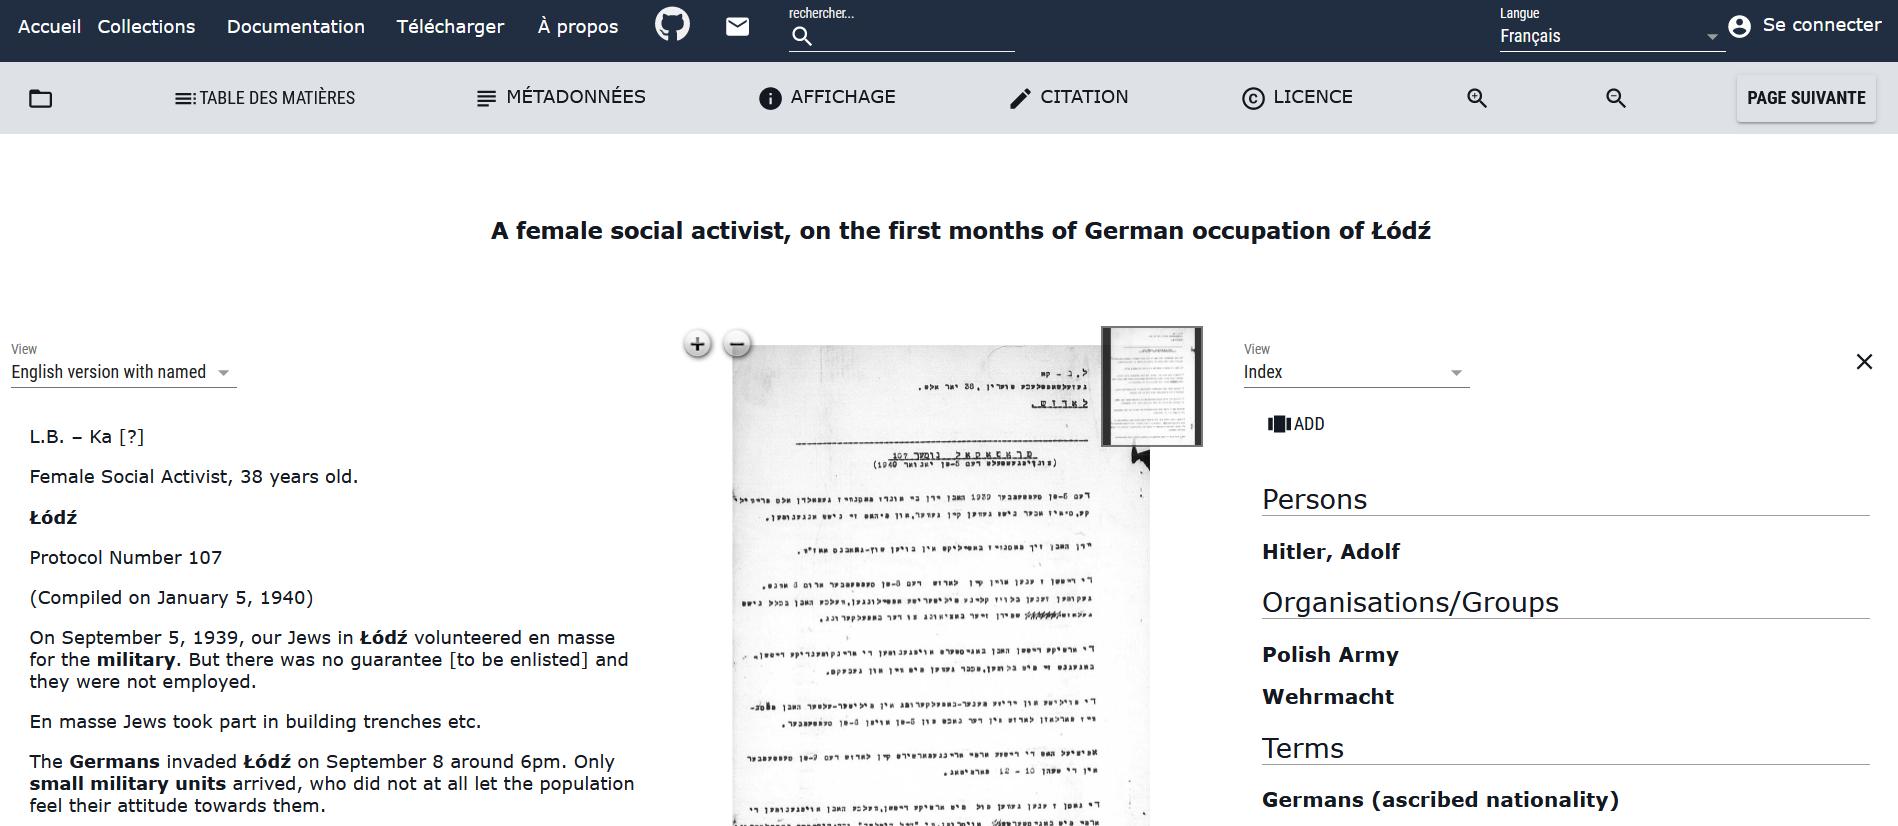
\includegraphics[width=\linewidth]{2-MAIN/images/discholed-document.png}
    \caption{Disposition horizontale avec TEI Publisher (Source~: DiScholEd)}
    \label{fig:doc-teipublisher}
\end{figure}

\begin{figure}[h]
    \centering
    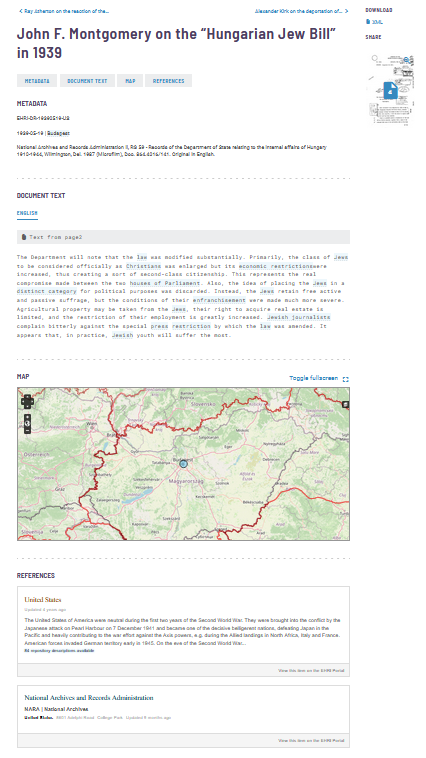
\includegraphics{2-MAIN/images/ehri-omeka.png}
    \caption{Diposition verticale avec Omeka (Source~: EHRI Online Editions)}
    \label{fig:ehri-omeka}
\end{figure}
    \chapter{EHRI sur l'application DiScholEd}
    % Une première expérimentation pour EHRI : l'application DiScholEd

\section{Une application pour publier les ego-documents}

\subsection{Qu'est-ce qu'un ego-document ?}
La mention d'\enquote{ego-document} apparaît dans les années 1950, utilisée par l'historien néerlandais Jacques Presser pour décrire les textes sur lesquels se basent ses recherches~: des journaux intimes, mémoires, autobiographies et de la correspondance personnelle (\enquote{\textit{Ego-Dokument}  \footcite[p.~46]{AltedVigil2022}}). Le terme \enquote{ego-document} est plus largement employé dans le monde anglophone~; en France, on entendra volontiers parler d'\enquote{écrits du for privé\footnote{Juliette Deloye, \enquote{For privé (écrits du)} dans VOCES, \textit{Vocabulaire pour l'Étude des Scripturalités}, Thomas Brunner (dir.), ARCHE UR3400 (Université de Strasbourg), édition électronique, 2019, \texttt{DOI~: \href{https://doi.org/10.34931/vvxh-5046}{10.34931/vvxh-5046}} (visité le 03/09/2023).}} ou d'\enquote{écriture de soi}. L'étude des ego-documents s'inscrit dans le courant historiographique de l'\enquote{Histoire par le bas} (\enquote{\textit{History From Below}}).


\subsection{Les collections publiées sur DiScholEd}
À ce jour, l'application DiScholEd\footcite{DiScholEd} compte sept collections. Nous présenterons ici les plus documentées par l'application. L'une d'entre elles, la collection \enquote{\textit{Early Holocaust Testimony} de l'EHRI}, nous intéressera particulièrement.  

\subsubsection*{Correspondance de Paul d'Estournelles de Constant}
Paul d’Estournelles de Constant (1852-1924) était un homme politique français. Il devient sénateur en 1905, fonction qu'il occupera jusqu'à sa mort. Prix Nobel de la paix, il a \oe{}uvré pour le maintien de la paix entre les pays, notamment avec la Grande-Bretagne et l'Allemagne. Le corpus est composé de sa correspondance pendant la Première Guerre mondiale. Paul d'Estournelles de Constant y apporte son point de vue en tant qu'élu, mais aussi en tant que citoyen et père de famille\footcite[collection \enquote{Correspondance de Paul d'Estournelles de Constant}, section \enquote{\textit{History of the Corpus}} (visité le 03/09/2023)]{DiScholEd}.  

\subsubsection*{Intellectuels Berlinois}
Le collection \enquote{Lettres et textes: Le Berlin intellectuel des années 1800} témoigne de la vie intellectuelle berlinoise de la fin du XVIII\ieme{} et du début du XIX\ieme{} siècle. Le corpus met en avant le développement du romantisme allemand et les relations que les cercles intellectuels berlinois entretenaient entre eux\footcite[collection \enquote{Lettres et textes: Le Berlin intellectuel des années 1800}, section \enquote{\textit{History of the Corpus}} (visité le 03/09/2023)]{DiScholEd}.

\subsubsection*{Catalogue des manuscrits d'Auguste Boeckh}
Auguste Boeckh (1785-1867) était un philologue allemand. Il a enseigné à l'université de Berlin, avant de devenir le doyen de la faculté des Arts et Sciences Humaines. La collection est composée du catalogue de ses manuscrits, réunis dans le cadre du projet \enquote{\textit{Boeckh-Nachlassprojekt\footcite[collection \enquote{Catalogue des manuscrits d'Auguste Boeckh}, section \enquote{\textit{History of the Corpus}} (visité le 03/09/2023)]{DiScholEd}}}.  



\section{La collection \enquote{\textit{Early Holocaust Testimony}} sur DiScholEd}
Le contenu de la collection \enquote{\textit{Early Holocaust Testimony}} sur DiScholEd est identique à celui de l'édition publiée avec Omeka\footnote{Consultable à l'adresse~: \texttt{\href{https://early-testimony.ehri-project.eu/}{https://early-testimony.ehri-project.eu/}}.}, seul l'affichage est différent. La simplicité de l'affichage proposé par TEI Publisher nous permet de présenter l'édition en donnant accès à l'utilisateur$\cdot$ice aux informations sur l'édition et sur l'EHRI, aux textes édités et aux index directement depuis la page d'accueil (Figure \ref{fig:ehri-discholed-accueil}). La présentation de la collection (section \enquote{Texts édités}) permet de naviguer directement dans toute la collection (Figure \ref{fig:ehri-discholed-collection}), alors que le site Omeka ne propose que d'explorer les exemples proposés par les éditeur$\cdot$ice$\cdot$s dans un premier temps.  

La disposition horizontale (Figure \ref{fig:doc-teipublisher}) permet d'afficher plusieurs vues d'une importance équivalente, alors que la présentation de la transcription sur Omeka se fait au détriment du fac-similé (Figure \ref{fig:ehri-omeka}), dont l'affichage nous semble tout particulièrement pertinent au sein d'une édition numérique de documents d'archives.

\begin{figure}[h]
    \centering
    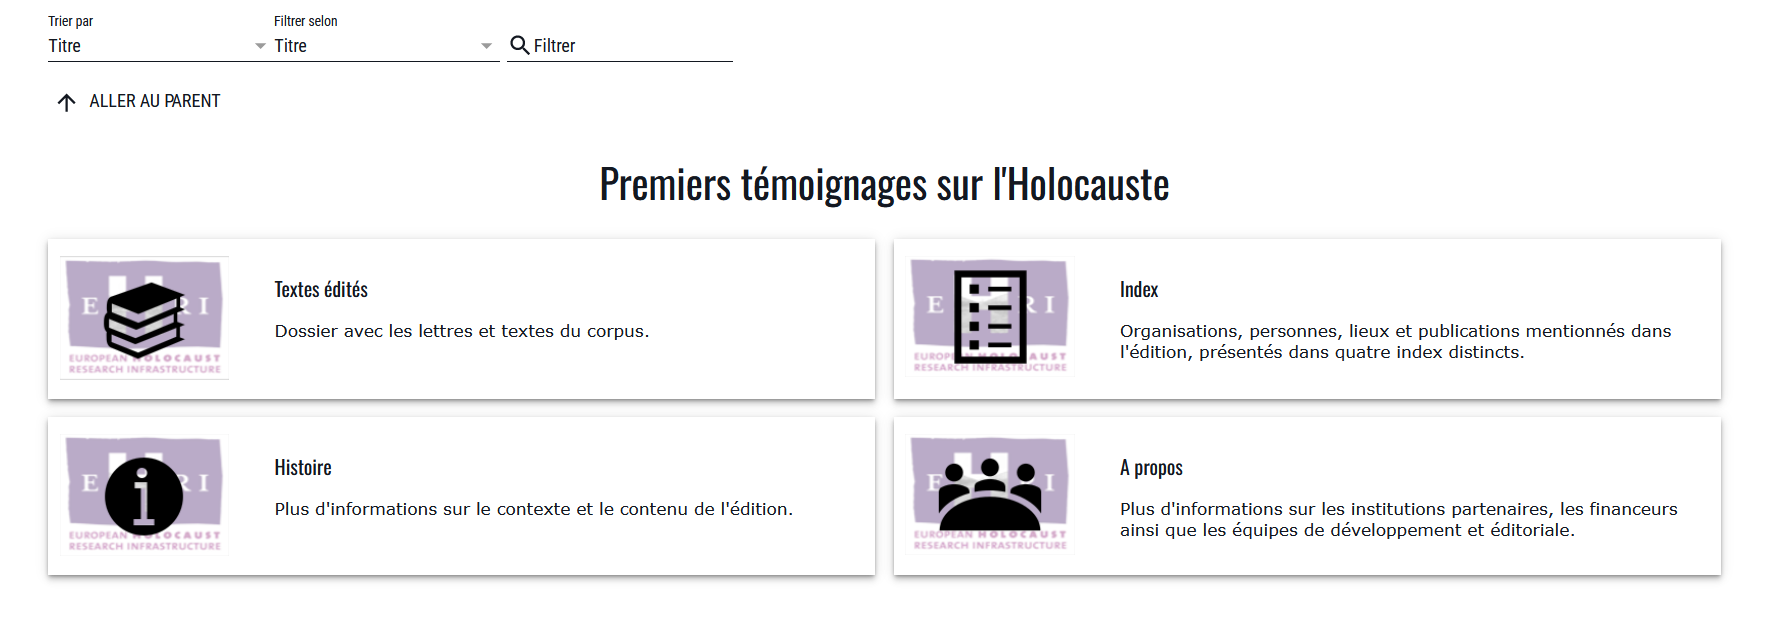
\includegraphics[width=1\linewidth]{2-MAIN/images/discholed-accueil.png}
    \caption{Page d'accueil de la collection sur DiScholEd}
    \label{fig:ehri-discholed-accueil}
\end{figure}

\begin{figure}[h]
    \centering
    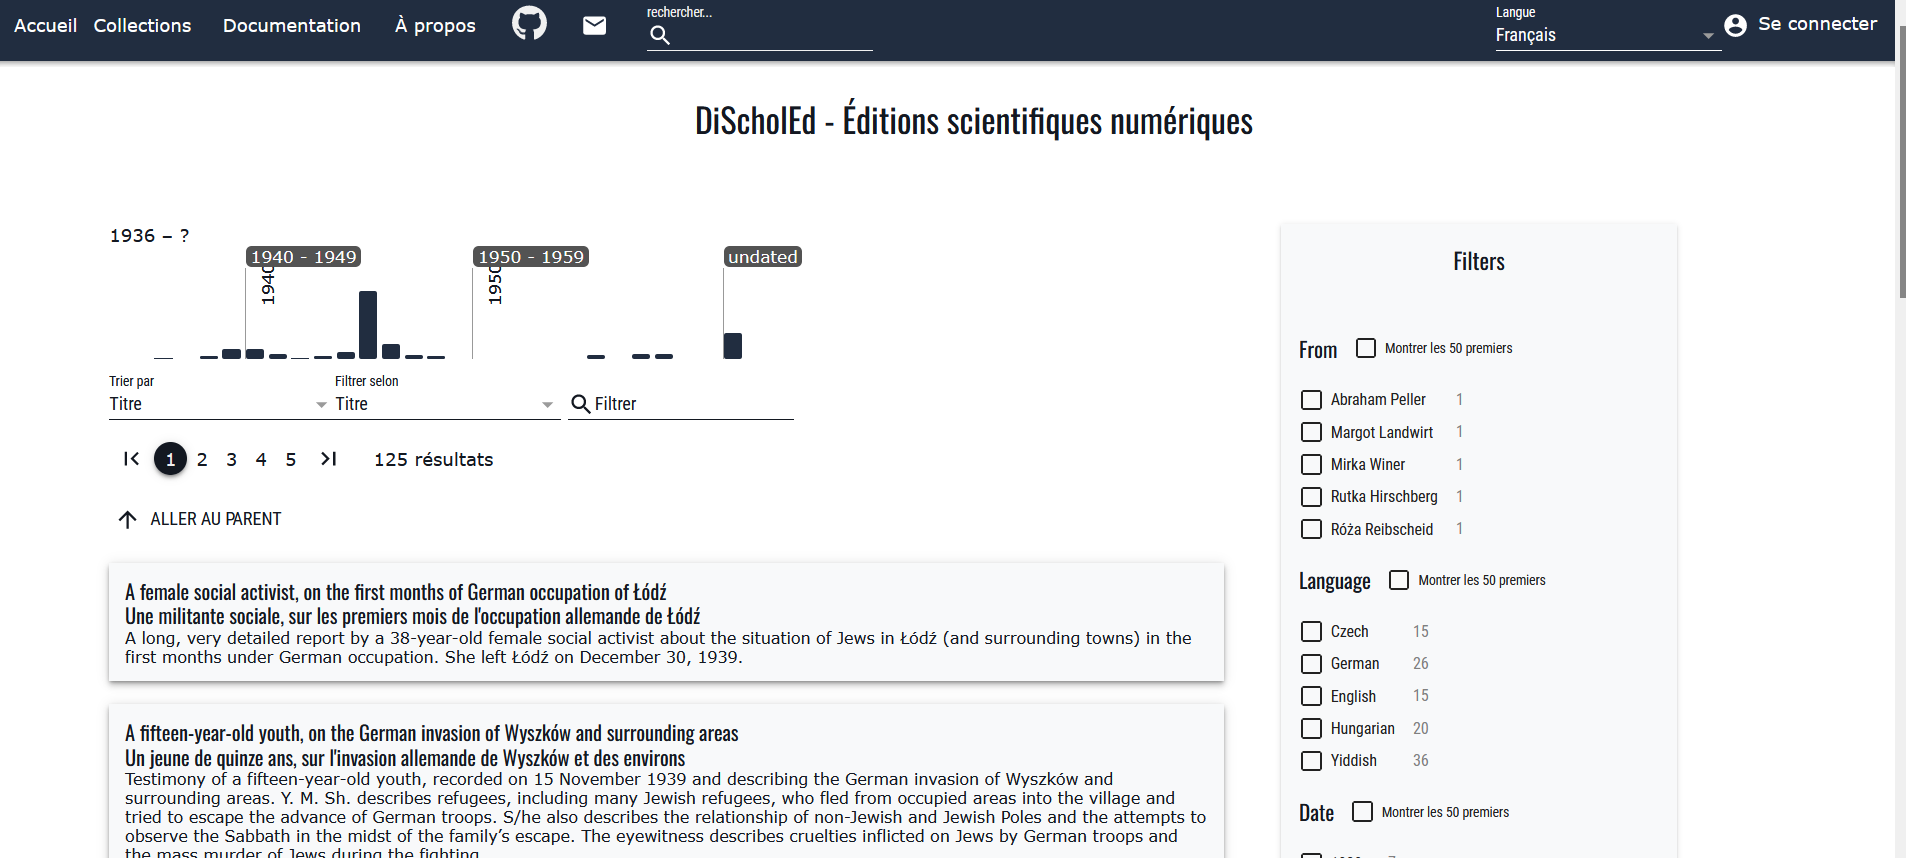
\includegraphics[width=1\linewidth]{2-MAIN/images/discholed-collection.png}
    \caption{Collection \enquote{\textit{Early Holocaust Testimony}} sur DiScholEd}
    \label{fig:ehri-discholed-collection}
\end{figure}

\bigskip
\bigskip
La publication de la collection \enquote{\textit{Early Holocaust Testimony}} sur DiScholEd a permis à l'équipe éditoriale du WP12 d'avoir une idée du rendu des éditions qu'elle pourrait y publier. La compatibilité naturelle de TEI Publisher avec les fichiers encodés en TEI permet à la communauté de développer des modules plus simples à incorporer à son projet. En outre, TEI Publisher dispose d'un outil d'annotation intégré dont la maîtrise optimiserait davantage le travail éditorial.
    \chapter{Transition vers une application dédiée}
    % Transition vers une application TEI Publisher pour les éditions en ligne EHRI

\section{Analyse des besoins}

\subsection{Profil des utilisateur$\cdot$ice$\cdot$s}
L'objectif principal de l'EHRI est de soutenir la recherche sur la Shoah, notamment en éditant des corpus thématiques. Les collections rassemblent des documents d'archives conservés dans les institutions partenaires du projet. De ce fait, les éditions de l'EHRI s'adressent plutôt à un public de chercheur$\cdot$euse$\cdot$s et d'étudiant$\cdot$e$\cdot$s, particulièrement en Histoire.


\subsection{Transposer les fonctionnalités d'Omeka}
Le cahier des charges des éditions EHRI publiées avec Omeka a été rigoureusement étudié\footcite{Ehri2018}. La transition vers TEI Publisher ne peut se faire sans s'assurer que les fonctionnalités dont dispose Omeka sont également disponibles dans TEI Publisher. Nous avons donc identifié quels étaient les principaux critères recherchés par l'équipe éditoriale, puis nous avons parcouru la liste des \textit{web components} de TEI Publisher pour établir une correspondance~:

\begin{itemize}
    \item La possibilité d'ajouter une documentation à propos de l'édition (module \texttt{pb-mark -down})~;
    \item Une barre de recherche (module \texttt{pb-search})~;
    \item Une recherche facettée (modules \texttt{pb-browse-docs} et \texttt{pb-custom-form})~;
    \item Une transcription lisible et sans distraction (modules \texttt{pb-view}, \texttt{pb-collapse}, \texttt{pb-grid} et \texttt{pb-grid-action}~;
    \item La possibilité de télécharger les fichiers dans plusieurs formats, principalement XML, PDF et ePub (module \texttt{pb-download})~;
    \item La génération de cartes interactives (modules \texttt{pb-leaflet}, \texttt{pb-geolocation}, \texttt{pb-map-icon} et \texttt{pb-map-layer})~;
    \item L'affichage d'informations contextuelles au survol de la transcription (modules \texttt{pb-highlight} et \texttt{pb-popover}).
\end{itemize}



\section{Création du prototype d'application}

\subsection{Des fonctionnalités supplémentaires}
Notre exploration des modules mis à disposition par TEI Publisher nous a permis d'établir une liste de fonctionnalités supplémentaires que l'application TEI Publisher dédiée à EHRI pourrait présenter~: 

\begin{itemize}
    \item Une application disponible en plusieurs langues (module \texttt{pb-lang})~;
    \item Une chronologie des documents (module \texttt{pb-timeline})~;
    \item Une navigation claire à l'intérieur de la collection (module \texttt{pb-paginate}), ce que toutes les éditions EHRI avec Omeka ne proposent pas~;
    \item Une navigation claire et simple à l'intérieur du document, notamment entre le fac-similé et la transcription (module \texttt{pb-navigation})~;
    \item La possibilité de zoomer aisément sur le fac-similé sans perte de qualité (module \texttt{pb-facsimile})~;
\end{itemize}

Certaines de ces fonctionnalités sont déjà disponibles sur l'application DiScholEd et pourront donc être facilement implémentées.


\subsection{Maquettes visuelles}
À partir des fonctionnalités décrites, nous avons proposé des maquettes visuelles pour le futur développement de l'application~: 

\begin{figure}[h]
    \centering
    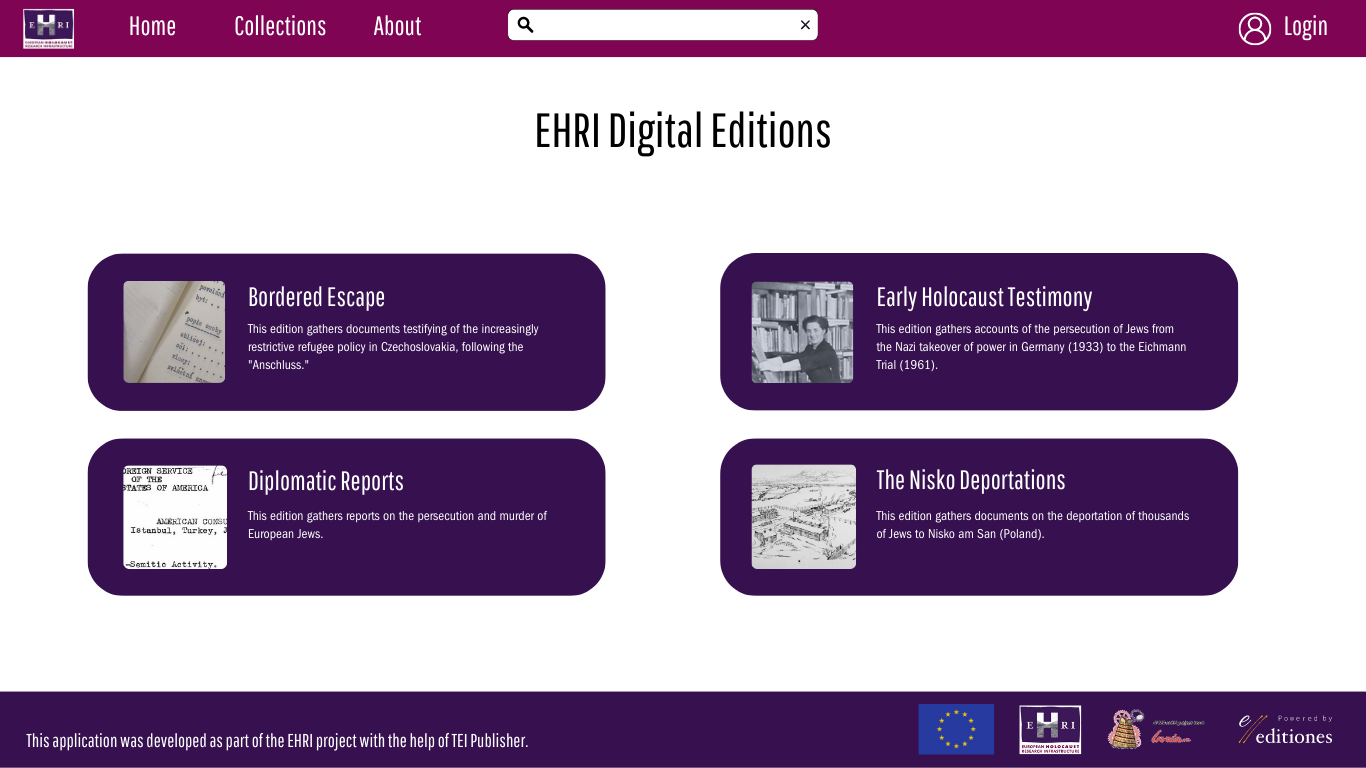
\includegraphics[width=0.55\linewidth]{2-MAIN/images/ehri-accueil.png}
    \caption{Maquette de la page d'accueil EHRI avec TEI Publisher}
    \label{fig:ehri-accueilmaquette}
\end{figure}

\begin{figure}[h]
    \centering
    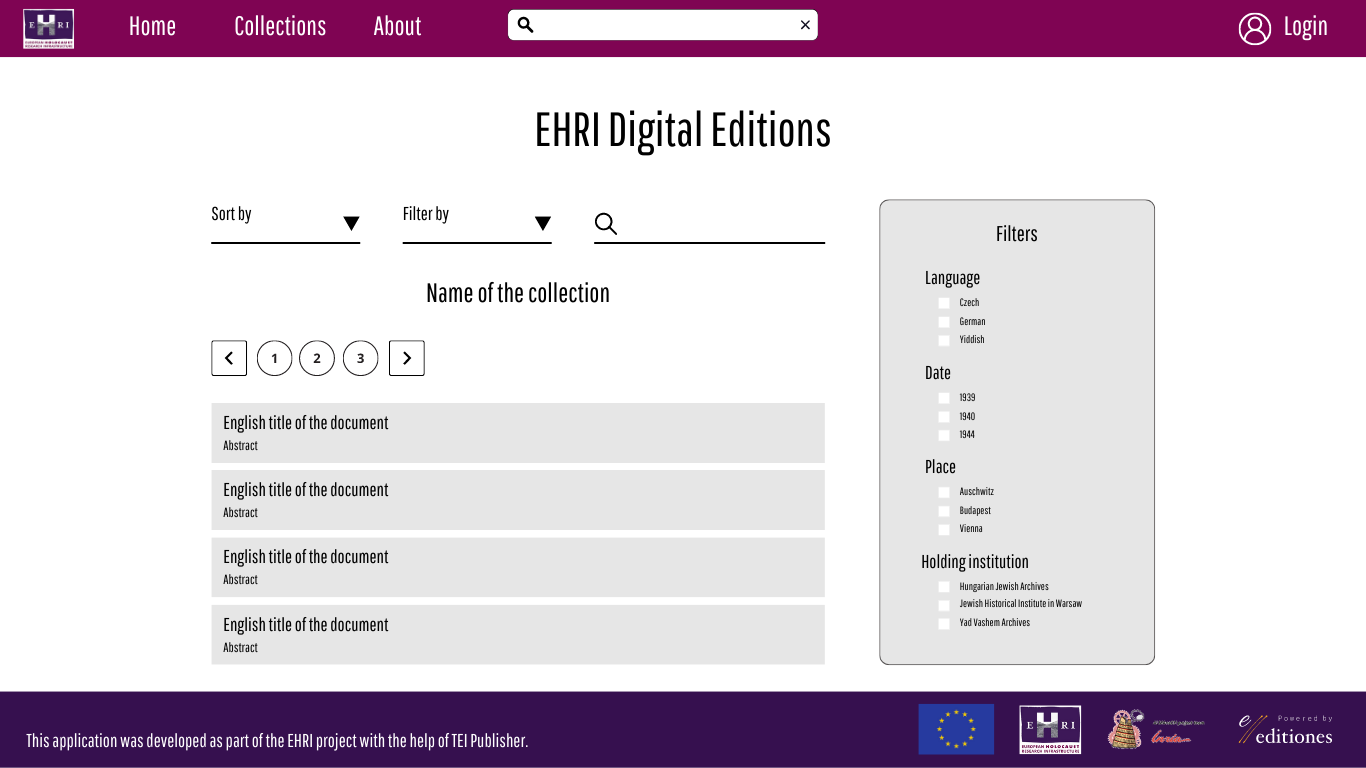
\includegraphics[width=0.55\linewidth]{2-MAIN/images/ehri-collection.png}
    \caption{Maquette de navigation dans la collection}
    \label{fig:ehri-collmaquette}
\end{figure}

\begin{figure}[h]
    \centering
    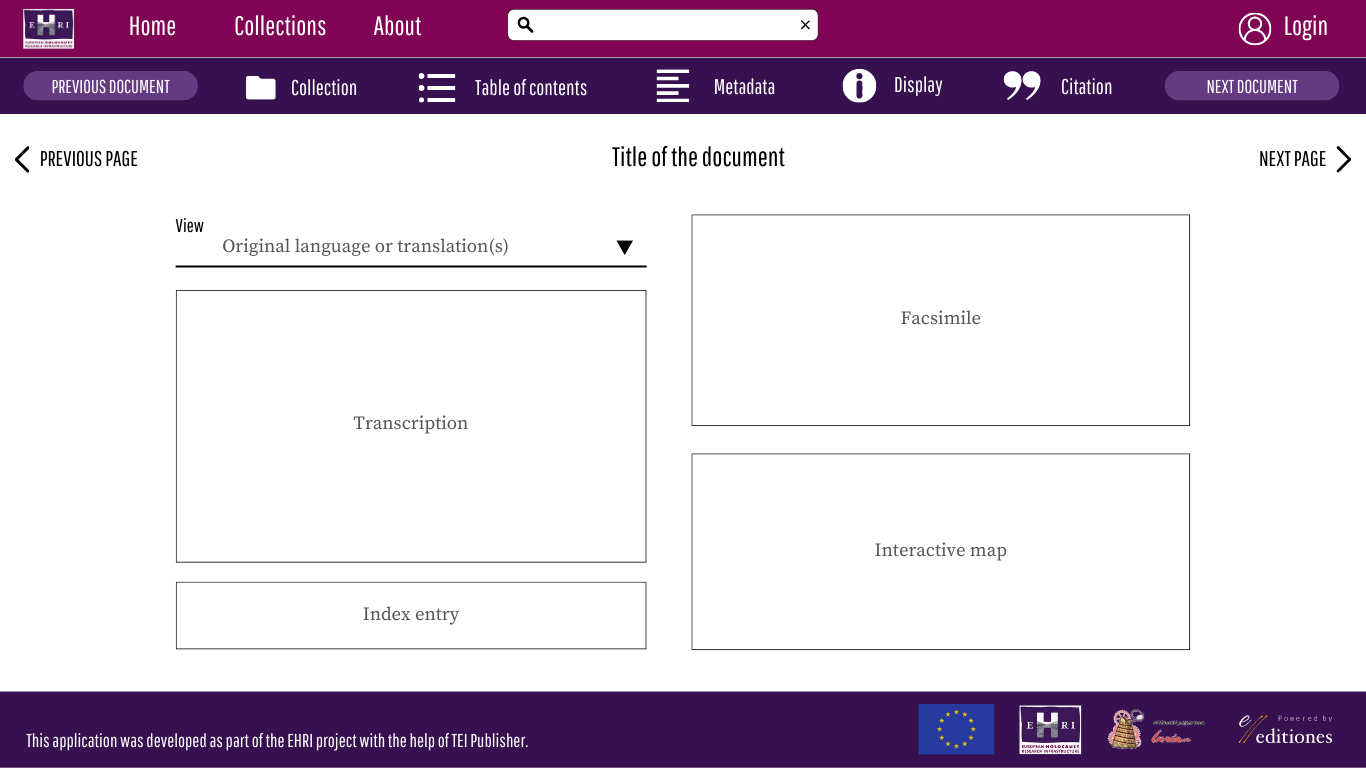
\includegraphics[width=0.55\linewidth]{2-MAIN/images/ehri-document.png}
    \caption{Maquette de l'affichage du document avec TEI Publisher}
    \label{fig:ehri-docmaquette}
\end{figure}

Notre équipe a commencé le développement de l'application TEI Publisher EHRI, dont le prototype devrait être présenté aux éditeur$\cdot$ice$\cdot$s du WP12 entre octobre et novembre prochains.

\begin{figure}[!h]
    \centering
    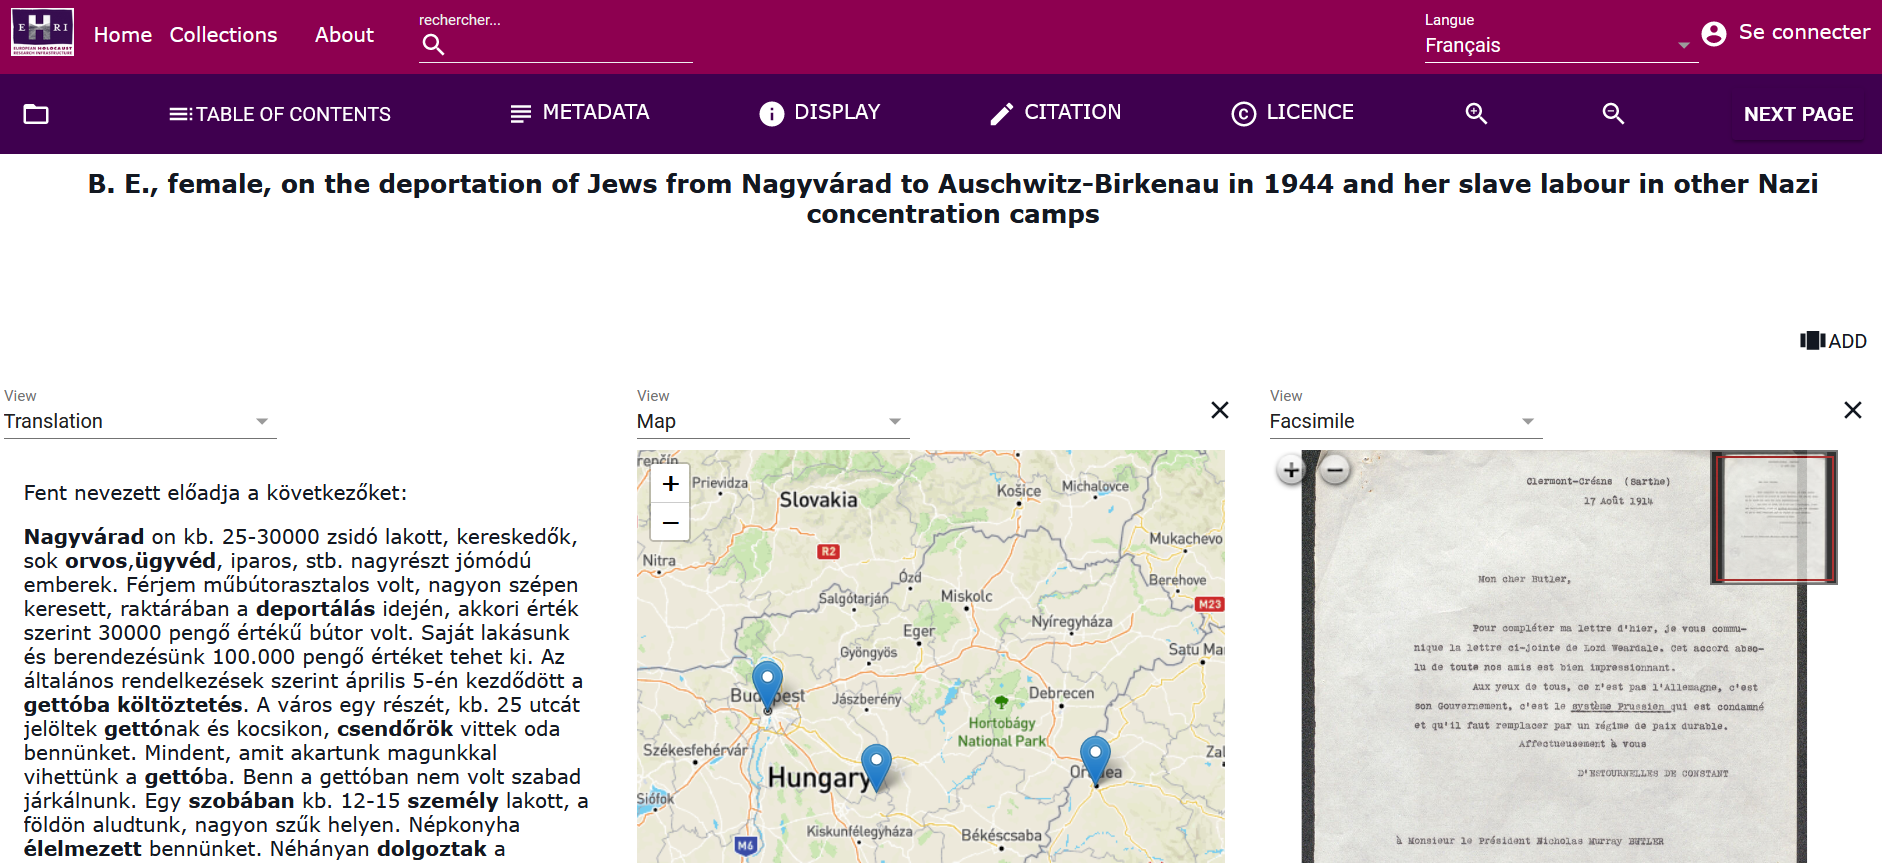
\includegraphics[width=1\linewidth]{2-MAIN/images/ehri-proofofconcept.png}
    \caption{Exemple de l'affichage d'un document sur l'application TEI Publisher EHRI}
    \label{fig:ehri-proofofconcept}
\end{figure}

Grâce à son affichage horizontal, TEI Publisher permet de profiter de trois vues simultanément sans perdre en confort de lecture (Figure \ref{fig:ehri-proofofconcept}). Les différentes vues sont par ailleurs modulables, c'est-à-dire que l'utilisateur$\cdot$ice peut choisir le nombre de vues souhaité et ce qu'elles affichent.

    % Conclusion
    \chapter*{Conclusion}
    \addcontentsline{toc}{chapter}{Conclusion}
    % Conclusion

La préparation d'une édition scientifique numérique est un processus long et passionnant. Leur publication permet de créer de formidables outils pour la recherche. Notre expérience nous a confirmé que la définition d'un modèle d'encodage est une étape primordiale afin d'assurer non seulement la validité et la conformité d'une édition, mais également l'uniformité à travers les collections. Le rôle de l'ingénieur$\cdot$e à cet égard est extrêmement important, notamment pour conseiller les chercheur$\cdot$euse$\cdot$s et les aider à naviguer parmi les outils, formats et standards.  

Les éditions de l'EHRI bénéficiant d'un aperçu de deux outils de publication, TEI Publisher et Omeka, les avantages de chacun d'eux ont pu être établis par rapport à un même corpus. Le développement de l'application TEI Publisher pour EHRI suit son cours, et les éditeur$\cdot$ice$\cdot$s pourront bientôt expérimenter l'outil d'annotation intégré à TEI Publisher, qui devrait encore davantage les aider dans leur travail éditorial.

    % Annexes
    \appendix
    \chapter{Glossaire}
    % Glossaire

\label{Glossaire}

Nous avons rédigé les définitions de ce glossaire à l'aide des références suivantes~:
\begin{itemize}
    \item \cite{Bensoussan2020}.
    \item \cite{Bruttmann2020}.
\end{itemize}

\bigskip
\bigskip

\begin{description}
    
    \item[Antisémitisme] Idéologie selon laquelle \enquote{le Juif} serait responsable de tous les maux. L'antisémitisme prend la forme de discrimination, voire de violences, à l'encontre des Juif$\cdot$ve$\cdot$s en raison de leur ethnie. 
    
    \item[Aryanisation] Processus visant à transférer la propriété d'une personne juive à un \enquote{aryen}. Le terme renvoie à une \enquote{opération de décontamination}. Il y a eu deux phases à l'aryanisation~: l'\enquote{aryanisation volontaire} et l'\enquote{aryanisation forcée}. Cette deuxième phase commence le 14 juin 1938 lorsque le ministre de l'Intérieur, Whilhelm Frick, décide de transférer les biens et propriétés juifs à l'État pour les revendre à crédit aux classes moyennes allemandes.      
    
    \item[Camp de concentration] (\textit{Konzentrationslager}). Symbole de la répression nazie, le camp de concentration est à l'origine un camp d'internement des opposants au régime. Le premier camp de concentration nazi est celui de Dachau en Allemagne.
    
    \item[Camp d'extermination] (Centre de mise à mort). Après les expérimentations de la mort par le gaz menés sur les malades mentaux lors de l'\enquote{Aktion T4}, la méthode est utilisée dans les camps pour exterminer le plus de victimes en un minimum de temps. Le premier camp d'extermination est celui de Chelmno, ouvert le 8 décembre 1941.
    
    \item[Déportation] Déplacement d'une personne ou d'un groupe de personne contre son gré. Durant la Shoah, les Juif$\cdot$ve$\cdot$s étaient déporté$\cdot$e$\cdot$s dans les ghettos, puis dans les camps de concentration et les camps d'extermination.
    
    \item[Groupes d'action spéciale] (\textit{Einsatzgruppen}). Unités mobiles du Reich allemand, chargées d'assassiner les Juif$\cdot$ve$\cdot$s et les commissaires politiques communistes. Au début, les groupes sont composés de presque 3~000 hommes, tous volontaires.
    
    \item[Émigration] Action volontaire de quitter son lieu de résidence ou son pays. L'objectif premier du régime nazi était de forcer les populations juives à émigrer hors d'Allemagne par le biais d'intimidations. Cette politique s'est soldée par un échec certain avec l'expansion du Reich, menant ensuite à la politique d'extermination de la population juive d'Europe.
        
    \item[Espace vital] (\textit{Lebensraum}). Concept du pangermanisme selon lequel le peuple allemand (comprendre les \enquote{aryens}) doit disposer d'un espace suffisant pour vivre. L'extension du territoire est vue comme une nécessité, ce qui permet au régime nazi de justifier ses invasions successives.
    
    \item[Génocide] Destruction partielle ou totale intentionnelle d'une population en raison de son ethnie ou de sa religion.

    \item[Gestapo] Abréviation de \enquote{\textit{Geheime Staatspolizei}}. Police politique de l'État nazi.
    
    \item[Ghetto] Quartier imposé aux Juif$\cdot$ve$\cdot$s par l'État. La population juive est forcée de vivre à l'écart de la population non-juive. Dans l'Allemagne nazie, les ghettos sont clôturés et constamment surveillés. La densité de population y est très élevée et les conditions de vies difficiles. Les autorités y pratiquent l'extermination par la faim et l'épidémie. Avec la \enquote{Solution finale}, les ghettos sont devenus une étape intermédiaire avant la déportation des Juif$\cdot$ve$\cdot$s vers les camps d'extermination.
    
    \item[Lois de Nuremberg] Distinguent la citoyenneté de la nationalité. \enquote{Le Juif} est défini par ses ascendants (au moins trois grands-parents juifs) et ne peut pas être citoyen. Les mariages et relations sexuelles entre Juif$\cdot$ve$\cdot$s et non-Juif$\cdot$ve$\cdot$s sont interdits.
    
    \item[Nazisme] Abréviation de national-socialisme. Idéologie antidémocratique et antimarxiste, nationaliste et pangermaniste.
    
    \item[Nuit de Cristal] (\textit{Kristallnacht}). Suite à l'assassinat d'un conseiller d'ambassade allemand le 7 novembre 1938 à Paris, Joseph Goebbels prononce un discours qui incite la population à une grande violence antisémite. Des \textit{pogroms} ont lieu partout~: 267 synagogues sont pillées, saccagées et incendiées, 7~500 magasins sont dévalisés ou détruits, les habitations des Juif$\cdot$ve$\cdot$s sont saccagées. La \enquote{Nuit de Cristal} dure jusqu'au 10 novembre, dans l'après-midi. Une centaine de Juif$\cdot$ve$\cdot$s sont assassinés, les femmes sont violées malgré l'interdit racial et les enfants juif$\cdot$ve$\cdot$s sont chassé$\cdot$e$\cdot$s des orphelinats. Près de 11~000 hommes sont arrêtés et envoyés à Dachau, et 10~000 à Buchenwald.
    
    \item[Pogrom] Terme russe signifiant 
    \enquote{dévastation} ou \enquote{destruction}. Désigne les violences antisémites commises par la population, incitée par le pouvoir en place. Le régime nazi a provoqué des \textit{pogroms} à de nombreuses reprises.
    
    \item[Question juive] Expression faisant originellement référence à la capacité des Juif$\cdot$ve$\cdot$s à s'intégrer en Europe occidentale. Pour le régime nazi, la \enquote{question juive} est un problème auquel il faut apporter une solution, qui consiste en l'extermination de la population juive.
    
    \item[Shoah] (Holocauste). Terme hébreu signifiant \enquote{catastrophe}, synonyme du terme \enquote{Holocauste} qui, à l'origine, fait référence à un sacrifice dans un but religieux. Le terme fait aujourd'hui référence au génocide des Juif$\cdot$ve$\cdot$s d'Europe par le régime nazi. Les anglophones emploient le terme \enquote{\textit{Holocaust}}, tandis que les francophones parlent de \enquote{Shoah}.
    
    \item[Solution finale] Projet d'extermination des Juif$\cdot$ve$\cdot$s d'Europe par le régime nazi. Ce \enquote{projet} est envisagé comme solution au \enquote{problème} posé par la \enquote{question juive}. La Solution finale accélère le processus entamé par l'enfermement des Juif$\cdot$ve$\cdot$s dans les ghettos et leur déportation dans les camps de concentration. Les premiers camps d'extermination sont créés dès 1941 et pratiquent la mort par le gaz et par balles.
    
    \item[Spoliation] Désigne la confiscation des biens possédés par les Juif$\cdot$ve$\cdot$s. La politique de spoliation orchestrée par le régime nazi a commencé par l'identification de tous les Juif$\cdot$ve$\cdot$s, qui a été suivie par une série de lois visant à les déposséder et anéantir leurs droits.
    
\end{description}
    \chapter{Chronologie de la persécution des Juifs}
    % Chronologie de l'histoire de la Shoah

Cette chronologie non exhaustive a été établie à partir des ressources suivantes~:
\begin{itemize}
    \item \cite{Bensoussan2020}.
    \item \cite{Bruttmann2020}.
    \item \cite{Memorial}.
\end{itemize}

\bigskip
\bigskip

\begin{description}

    \item[XIII\ieme{} siècle] Création des premiers ghettos et premières grandes migrations de l'Europe occidentale vers l'Europe de l'Est, en particulier vers la Pologne et la Lituanie.
    
    \item[1215] Le IV\ieme{} concile du Latran impose aux Juifs le port d'un signe distinctif~: la \enquote{rouelle} (petit pièce de tissu jaune).
    
    \item[15 novembre 1879] Heinrich Gothard von Treitschke publie un article antisémite dans les \textit{Annales prussiennes}, dont les Nazis reprendront la formule~: \enquote{Les Juifs sont notre malheur~!}.
    
    \item[1881-1882] En Russie, les \textit{pogroms} accélèrent l'émigration des Juifs de Russie.
    
    \item[Années 1900] Montée du darwinisme social et de l'idéologie eugéniste en Allemagne.

    \item[5 janvier 1919] Création du Parti ouvrier allemand, qui devient le Parti national-socialiste des travailleurs allemands (NSDAP) en 1921.
    
    \item[Années 1920] Montée de la xénophobie et de l'antisémitisme. La défaite de l'Allemagne à l'issue de la Première Guerre mondiale pousse la classe moyenne allemande vers le nationalisme d'extrême-droite.
    
    \item[1919-1921] Nombreux \textit{pogroms} en Pologne.
    
    \item[24 février 1920] Premier programme politique du NSDAP. Il entend retirer aux Juifs la citoyenneté allemande et réduire leurs droits à ceux des étrangers. Un point révoque l'accès aux emplois de la fonction publique pour les Juifs, et un autre souhaite expulser les Juifs entrés en Allemagne après le 2 août 1914.
    
    \item[18 juillet 1925] Publication de \textit{Mein Kampf} (Adolf Hitler).
    
    \item[30 janvier 1933] Adolf Hitler est appelé à la Chancellerie.
    
    \item[5 mars 1933] Élections législatives anticipées. Le NSDAP obtient 44~\%{} des suffrages.
    
    \item[27 février 1933] Incendie du Reichstag. 
    
    \item[22 mars 1933] Ouverture du premier camp de concentration à Dachau (Allemagne).
    
    \item[23 mars 1933] Hitler obtient les pleins pouvoirs.

    \item[Avril 1933] Les fonctionnaires juifs sont révoqués et les avocats juifs sont radiés du barreau.
    
    \item[26 avril 1933] Création de la Gestapo.

    \item[14 juillet 1933] Loi sur la stérilisation forcée. Les personnes atteintes de \enquote{maladies héréditaires} (physiques ou mentales) et les criminels \enquote{irrécupérables et dangereux} sont stérilisés avec l'appui des psychiatres.

    \item[14 juillet 1933] Le NSDAP devient le seul parti autorisé en Allemagne.

    \item[25 août 1933] L'Accord de \enquote{\textit{haavara}} (de l'hébreu \enquote{transfert}) permet de négocier le départ de 60~000 Juifs vers la Palestine.

    \item[29 juin 1934] Nuit des longs couteaux.
    
    \item[Juillet 1934] Création de l'Inspection des camps de concentration.

    \item[1\ier{} août 1934] Hitler se proclame \enquote{Führer} et Chancelier du Reich.
    
    \item[15 septembre 1935] Lois de Nuremberg. Séparation physique des Juifs des autres Allemands.

    \item[7 mars 1936] Entrée de la Wehrmacht en Rhénanie (zone démilitarisée par le Traité de Versailles en 1919).

    \item[12 juillet 1936] Ouverture du camp de concentration d'Oranienburg-Sachsenhausen.

    \item[15 juillet 1937] Ouverture du camp de concentration de Buchenwald.
    
    \item[Mars 1938] Aux États-Unis, 82\%{} de la population s'oppose à l'accueil de réfugiés juifs venus d'Allemagne et d'Autriche.
    
    \item[12--13 mars 1938] Annexion de l'Autriche (\textit{Anschlu\ss{}})

    \item[Avril 1938] Création d'un centre d'émigration juive à Vienne, dirigé par Adolf Eichmann. En six mois, le quart de la communauté juive est expulsée.
    
    \item[26 avril 1938] Les Juifs doivent déclarer tous leurs biens.
    
    \item[Mai 1938] Première législation antisémite en Hongrie.
    
    \item[14 juin 1938] Début de l'aryanisation forcée.

    \item[Juillet 1938] Les médecins juifs doivent demander l'autorisation d'exercer et limiter leur pratique à une patientèle juive.
    
    \item[6--15 juillet 1938] La conférence d'Évian réunit trente-deux états pour répondre à la question des réfugiés juifs. La Hongrie, la Roumanie et la Pologne envoient des \enquote{observateurs}. \enquote{Nul ne conteste à l'Allemagne sa souveraineté à l'égard de ses nationaux}.

    \item[Août 1938] Les Juifs doivent ajouter un prénom de marquage à leur prénom courant~: \enquote{Israël} pour les hommes, \enquote{Sara} pour les femmes.
    
    \item[8 août 1938] Ouverture du camp de concentration de Mauthausen (Autriche).

    \item[30 septembre 1938] Accords de Munich.
    
    \item[9--10 novembre 1938] Nuit de Cristal (\textit{Kristallnacht}).    
    
    \item[Décembre 1938] En Autriche, les Juifs perdent leur permis de conduire.

    \item[3 décembre 1938] Les propriétaires juifs reçoivent l'ordre de vendre tous leurs biens restants.
    
    \item[31 décembre 1938] Les travailleurs indépendants juifs doivent cesser toute activité.

    \item[Janvier 1939] Création du \enquote{Bureau central pour l'émigration des Juifs} à Berlin, dirigé par Reinhard Heydrich.
    
    \item[Mars 1939] La Suisse ferme ses frontières aux réfugiés juifs.

    \item[15 mars 1939] Invasion de la Tchécoslovaquie et violation des Accords de Munich.

    \item[Avril 1939] En Autriche, les locataires juifs perdent tous leurs droits face à leurs propriétaires.
    
    \item[Mai 1939] Recensement général de la population allemande. Les fiches des Juifs sont marquées de la lettre \enquote{J}.
    \item[Mai 1939] Ouverture du camp de concentration de  Ravensbrück.
    
    \item[Septembre 1939] Couvre-feu à 20h pour les Juifs uniquement.

    \item[1\ier{} sepembre 1939] Invasion de la Pologne par l'Allemagne.

    \item[25 septembre 1939] La Pologne est divisée en quatre zones réparties entre l'Allemagne, l'URSS et la Lituanie.
    
    \item[27 septembre 1939] Début de l'\enquote{Aktion T4} à l'asile de Kocborowo (Pologne).

    \item[Octobre 1939] Début des déportations vers Nisko (Pologne).
    
    \item[8 octobre 1939] Création du ghetto de Piotrkow.
    
    \item[9 octobre 1939] Début du recensement des malades mentaux.
    
    \item[26 octobre 1939] Instauration du travail forcé pour les personnes âgées de 14 à 60 ans dans le \enquote{gouvernement général} (zone de Pologne occupée par l'Allemagne).

    \item[28 novembre 1939] Créations des \enquote{Conseils juifs} dans le \enquote{gouvernement général}. La communauté juive prend elle-même en charge les tâches administratives liées au recensement, à la spoliation et à la déportation de sa population.
    
    \item[Décembre 1939] Exclusion des Juifs allemands des distributions spéciales de nourritures.

    \item[11 décembre 1939] Tout changement de domicile est interdit aux Juifs polonais.

    \item[Mars 1940] Identification des Juifs par un \enquote{J} sur leur carte alimentaire.

    \item[20 avril 1940] Création du ghetto de Lodz.
    
    \item[9 avril 1940] Invasion du Danemark et du sud de la Norvège.

    \item[27 avril 1940] Ouverture du camp de concentration d'Auschwitz.

    \item[2 octobre 1940] Création du ghetto de Varsovie.

    \item[Janvier 1941] Création des \enquote{\textit{Einsatzgruppen}}.
    
    \item[3 mars 1941] Création du ghetto de Cracovie.

    \item[24 mars 1941] Création du ghetto de Lublin.
    
    \item[Avril 1941] Début de l'\enquote{Aktion 14f13}. Mise à mort des détenus incapables de travailler dans les camps de concentration.

    \item[29 juin 1941] Opération Barbarossa (invasion de la Russie).

    \item[15 août 1941] Heinrich Himmler se rend à Minsk et décide d'expérimenter le meurtre à l'aide des camions à gaz, déjà utilisés pour l'assassinat des malades mentaux.

    \item[24 août 1941] Hitler annonce la fin de l'\enquote{Aktion T4}.
    
    \item[Septembre 1941] Les Juifs allemands de plus de 6 ans doivent porter l'étoile de David sur le côté gauche de leur vêtement. Ils ne peuvent plus quitter leur commune de résidence.

    \item[5--6 septembre 1941] Les prisonniers de guerre soviétiques sont assassinés par le gaz Zyklon B à Auschwitz.

    \item[16 et 18 septembre 1941] Premiers essais des camions à gaz à Mohilev et à Minsk (Biélorussie).

    \item[29 septembre 1941] Massacre de Babi Yar (Ukraine).

    \item[Octobre 1941] Le ghetto de Lodz devint un centre de transit pour les Juifs déportés du Reich.

    \item[1\ier{} octobre 1941] Début des travaux visant à transformer le Birkenau (Auschwitz) en camp d'extermination.

    \item[23 octobre 1941] L'Europe allemande est définitivement fermée à l'émigration juive.

    \item[1\ier{} novembre 1941] Construction du centre de mise à mort de Belzec (Pologne).

    \item[3 novembre 1941] Essais des camions à gaz à Sachsenhausen.

    \item[8 novembre 1941] Création du ghetto de Lwow (Ukraine).

    \item[24 novembre 1941] Ouverture du camp de concentration de Terezin (République Tchèque).

    \item[7 décembre 1941] Attaque de Pearl Harbor.

    \item[8 décembre 1941] Ouverture du camp d'extermination de Chelmno, près de Lodz. Début des exterminations par le gaz.
    
    \item[20 janvier 1942] Conférence de Wansee. Début de la \enquote{Solution finale}.

    \item[17 ars 1942] Ouverture du camp d'extermination de Belzec (Pologne).

    \item[7 mai 1942] Ouverture du camp d'extermination de Sobibor (Pologne).

    \item[22 juillet 1942] Ouverture du camp d'extermination de Treblinka (Pologne) et déportation des Juifs du ghetto de Varsovie.

    \item[13--14 mars 1943] Liquidation du ghetto de Cracovie.

    \item[19 avril 1943 -- 16 mai 1943] Révolte du ghetto de Varsovie.

    \item[21 juin 1943] Décision de liquider tous les ghettos de Pologne.

    \item[3 novembre 1943] Début de l'Opération \enquote{\textit{Erntefest}} (\enquote{Fête de la Moisson}~: extermination Juifs de Lublin (environ 45000).

    \item[19 mars 1944] Invasion de la Hongrie.

    \item[Août 1944] Liquidation du ghetto de Lodz et déportation des survivants à Auschwitz.

    \item[30 octobre 1944] Déportation des Juifs de Theresienstadt vers Auschwitz.

    \item[27 janvier 1945] Libération d'Auschwitz.

    \item[30 avril 1945] Suicide d'Adolf Hitler.

    \item[7 mai 1945] Capitulation de l'Allemagne.
    
    \item[18 octobre 1945 -- 1\ier{} octobre 1946] Procès de Nuremberg.

\end{description}
    \chapter{Tableau récapitulatif d'encodage}
    % Tableau récapitulatif des balises et attributs utilisés par les éditions EHRI

\label{Tableau}

\begin{figure}[ht]
    \centering
    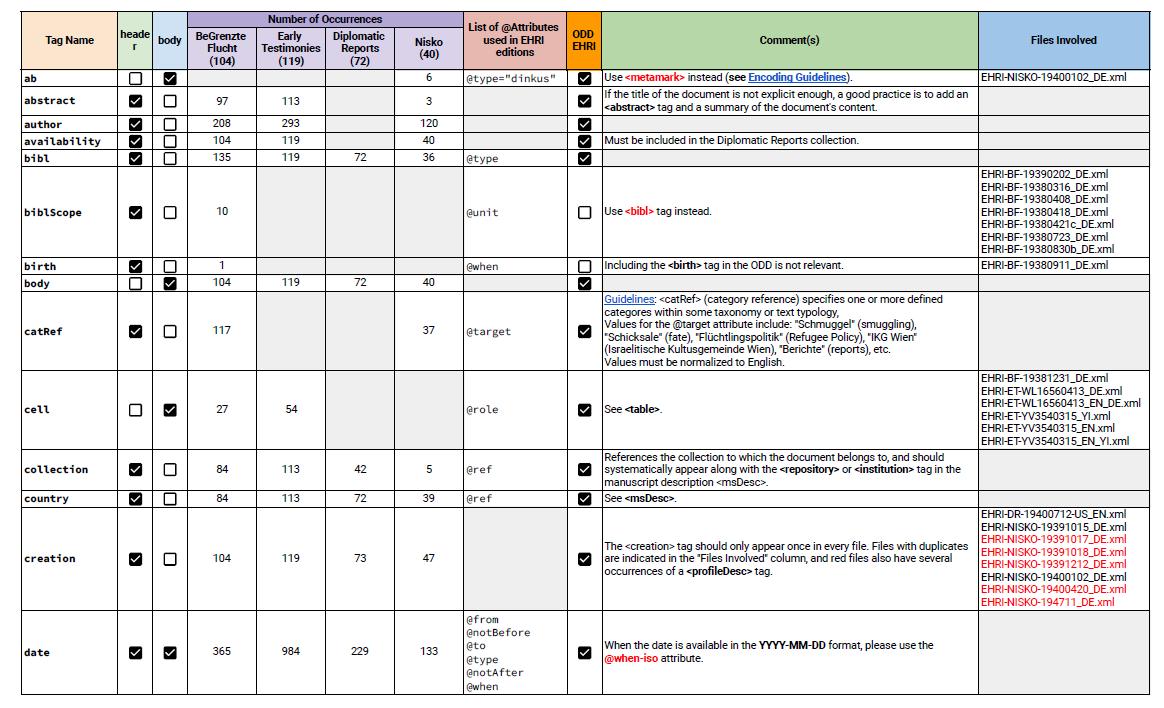
\includegraphics[width=1\linewidth]{3-ANNEXES/images/encodage-ehri-1.png}
    \caption{Balises et attributs utilisés par les éditions EHRI (1/5)}
    \label{fig:TableauRecap1}
\end{figure}  

\begin{figure}[ht]
    \centering
    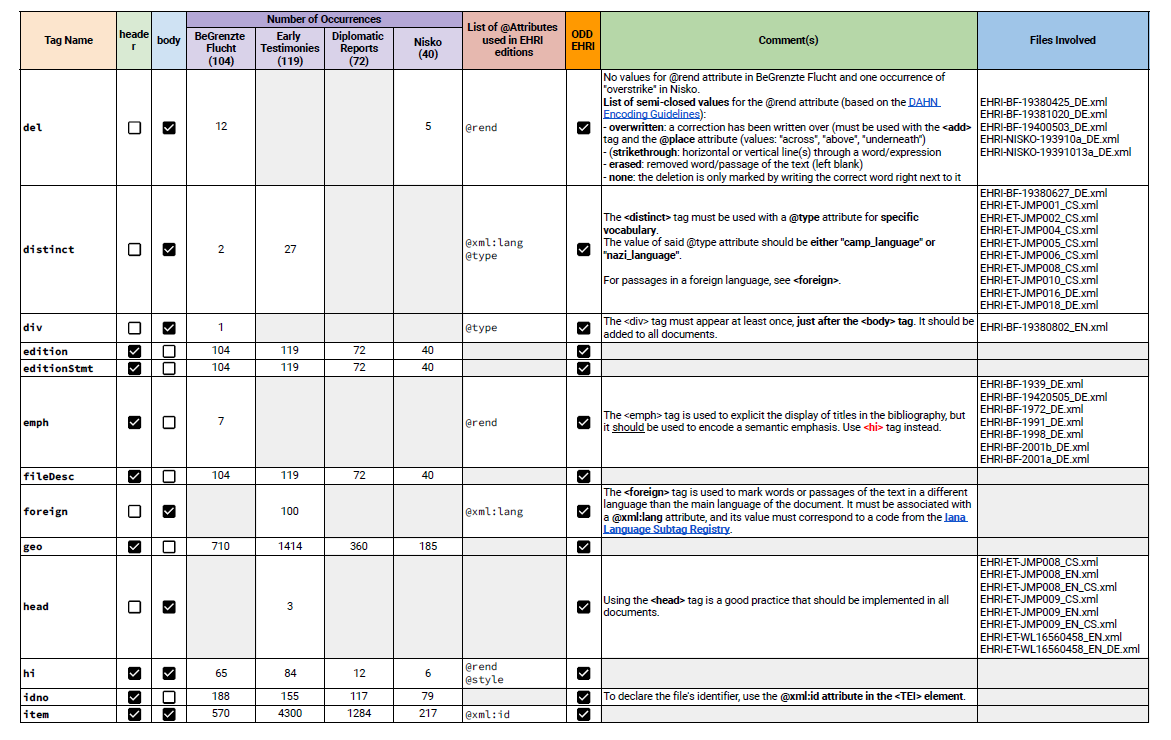
\includegraphics[width=1\linewidth]{3-ANNEXES/images/encodage-ehri-2.png}
    \caption{Balises et attributs utilisés par les éditions EHRI (2/5)}
    \label{fig:TableauRecap2}
\end{figure}  

\begin{figure}[ht]
    \centering
    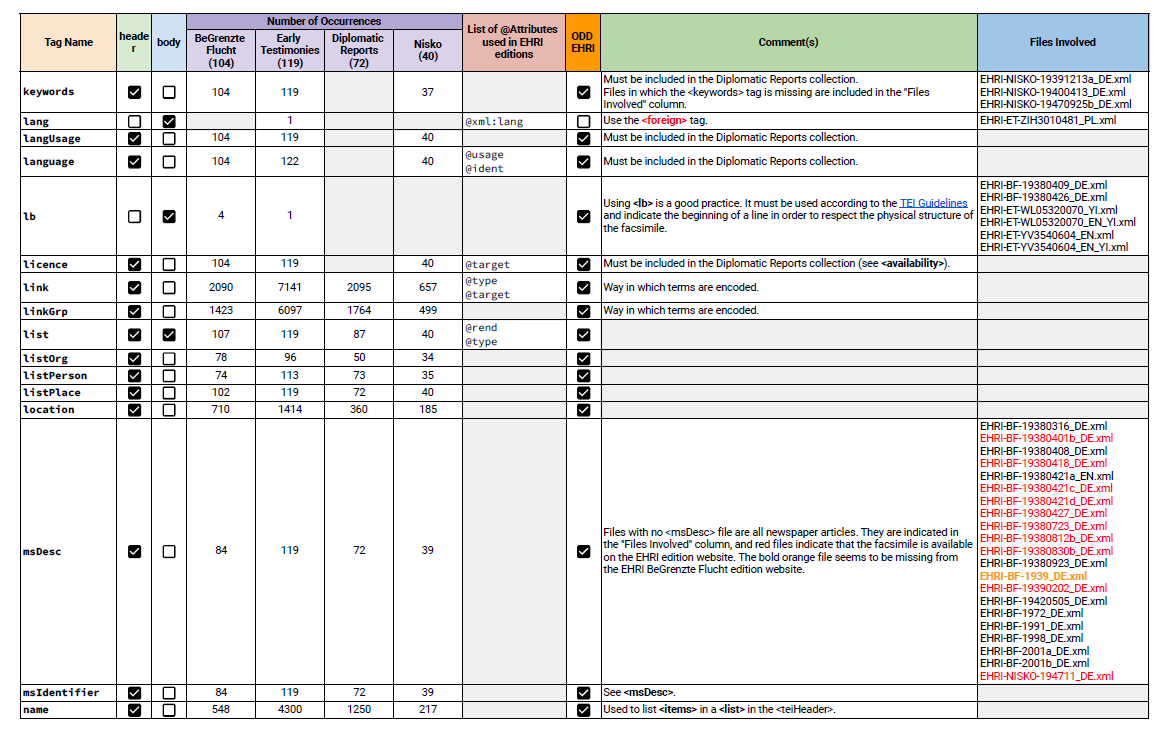
\includegraphics[width=1\linewidth]{3-ANNEXES/images/encodage-ehri-3.png}
    \caption{Balises et attributs utilisés par les éditions EHRI (3/5)}
    \label{fig:TableauRecap3}
\end{figure}  

\begin{figure}[ht]
    \centering
    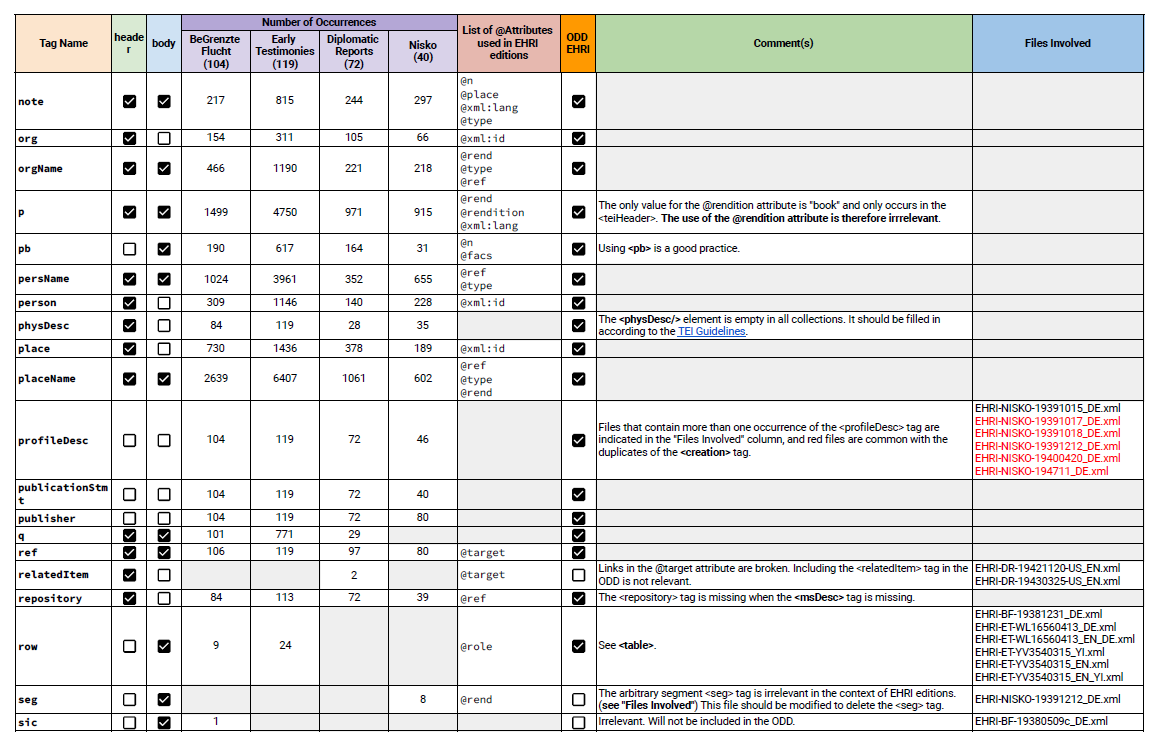
\includegraphics[width=1\linewidth]{3-ANNEXES/images/encodage-ehri-4.png}
    \caption{Balises et attributs utilisés par les éditions EHRI (4/5)}
    \label{fig:TableauRecap4}
\end{figure}  

\begin{figure}[ht]
    \centering
    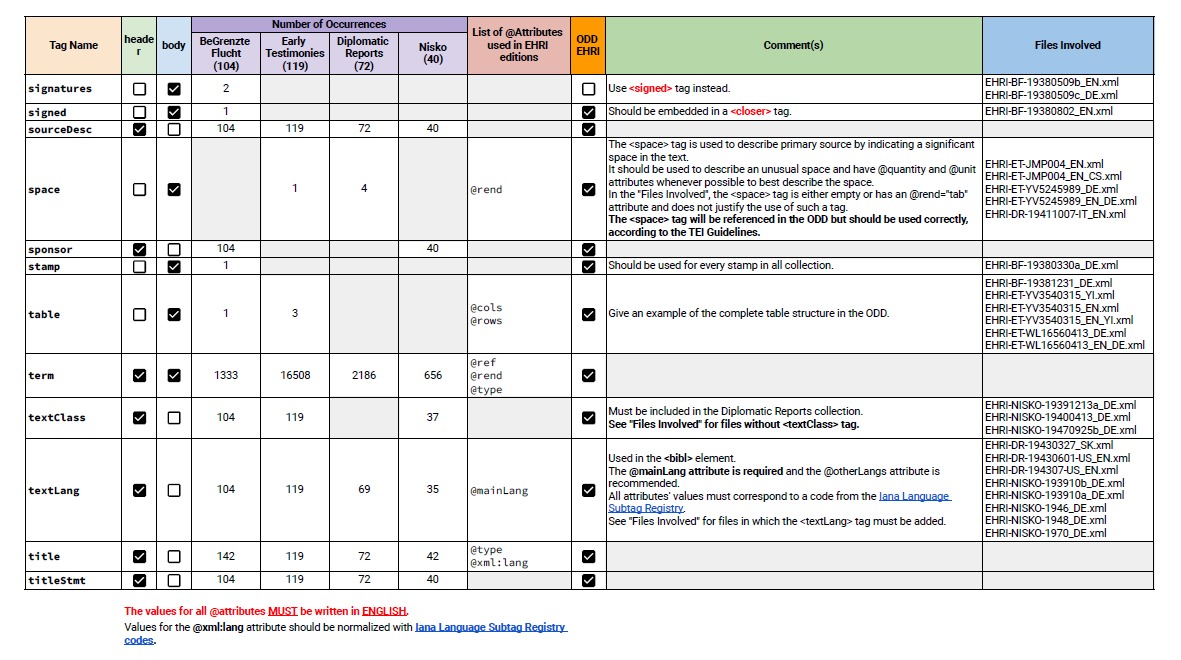
\includegraphics[width=1\linewidth]{3-ANNEXES/images/encodage-ehri-5.png}
    \caption{Balises et attributs utilisés par les éditions EHRI (5/5)}
    \label{fig:TableauRecap5}
\end{figure}  
    \chapter{Encodage des métadonnées}
    % Structure du <teiHeader> pour l'encodage des éditions EHRI

\label{Metadonnees}

\begin{minted}[linenos, breaklines=true]{xml}
<teiHeader>
    <fileDesc>
        <titleStmt>
            <title xml:lang="en"/>
            <title xml:lang=""/>
            <principal>
                <affiliation>
                    <orgName ref="https://www.ehri-project.eu">European Holocaust Research Infrastructure</orgName>
                </affiliation>
            </principal>
            <respStmt>
                <resp/>
                <persName/>
            </respStmt>
        </titleStmt>
        <publicationStmt>
            <authority>
                <ref target="https://www.ehri-project.eu">European Holocaust Research Infrastructure</ref>
            </authority>
            <availability>
                <licence target="http://creativecommons.org/licenses/by-sa/4.0">
                Attribution-ShareAlike 4.0 International
            </licence>
            </availability>
        </publicationStmt>
        <seriesStmt>
            <title ref="{link to the online edition}"/>
        </seriesStmt>
        <sourceDesc>
            <msDesc>
                <msIdentifier>
                    <institution>
                        <orgName/>
                        <address>
                            <street>
                                <num/>
                            </street>
                            <postCode/>
                            <settlement/>
                            <country/>
                        </address>
                    </institution>
                    <collection/>
                    <idno/>
                </msIdentifier>
                <physDesc>
                    <p/>
                </physDesc>
            </msDesc>
            <bibl>
                <textLang/>
            </bibl>
        </sourceDesc>
    </fileDesc>
    <encodingDesc>
        <projectDesc>
            <p xml:lang="en"/>
        </projectDesc>
    </encodingDesc>
    <profileDesc>
        <creation>
            <origDate when=""/>
            <origPlace ref="{GeoNames link}"/>
            <persName ref="{EHRI entity}"/>
        </creation>
        <textClass>
            <catRef target="{link to EHRI portal}"/>
            <keywords>
                <term/>
            </keywords>
        </textClass>
        <langUsage>
            <language ident=""/>
        </langUsage>
        <abstract>
            <p xml:lang="en"/>
        </abstract>
    </profileDesc>
    <revisionDesc>
        <change when="" who="{}"/>
    </revisionDesc>
</teiHeader>
\end{minted}
    \chapter{Extrait du script de recherche}
    % Extrait du script de recherche

\label{Script}

\begin{minted}[linenos, breaklines=true]{python}    
    import os  # Allows interaction with the computer, regardless of its operating system.
    import sys  # Allows for the argument to be called directly from the command line.
    from bs4 import BeautifulSoup
  
    def parse(corpus):
        """ Parses the given corpus.
        Parameter
        ---------
        corpus
           Absolute path for the corpus.
           Corresponds to "arg1" in the command line.
        """
        for root, dirs, files in os.walk(corpus):
            for filename in files:
                with open(os.path.join(root, filename), 'r', encoding='UTF-8') as xml_file:
                # Opens the files in 'read' mode and stores the opened file in a variable called 'xml_file'.
                    xml_content = xml_file.read()
                    # The 'xml_content' variable stores the content of the file opened in 'xml_file' with the '.read()' method.
                    soup = BeautifulSoup(xml_content, 'xml')
                    # Creates a 'soup' object, which parses 'xml_content' with the XML parser included in the BeautifulSoup library.
                    yield filename, soup
                    # The 'yield' statement suspends the execution of the function to return a result, and then resumes execution instead of starting over every time.

   
    def missing_tag(tag):
        """ Finds the files from which the element is missing.
        Parameter
        ---------
        tag : str
            Name of the researched element, between quotation marks.    
        Returns
        -------
        set()
            Set containing the names of the files from which the given element is missing.
        """
        files_missing_tag = set()
        for filename, soup in parse(sys.argv[1]):
            # Uses the 'parse' function to parse the corpus provided by 'arg1' in the command line.
            if not soup.find_all(tag):
                files_missing_tag.add(filename)
                # Adds the name of the file to the set if the '.find_all()' method does not find any occurrence.
                print(filename)
    # Example --> missing_tag("catRef")
\end{minted}

    \backmatter
	
 % Figures
    \listoffigures
    
    % Table des matières
    \tableofcontents
    
\end{document}